\documentclass[a4paper,12pt]{article}
\usepackage[utf8]{inputenc}
\usepackage[ngerman]{babel}
\usepackage[T1]{fontenc}
\usepackage{csquotes}
\usepackage{amsmath}
\usepackage{amssymb}
\usepackage{amsthm}
\usepackage{geometry}
\usepackage{graphicx}
\usepackage[hidelinks]{hyperref}
\usepackage{listings}
\usepackage{xcolor}
\usepackage{enumitem}
\usepackage{booktabs}
\usepackage{array}
\usepackage{caption}

\geometry{margin=2.5cm}

\theoremstyle{definition}
\newtheorem{definition}{Definition}
\newtheorem{beispiel}{Beispiel}
\newtheorem{satz}{Satz}
\newtheorem{lemma}{Lemma}
\newtheorem{bemerkung}{Bemerkung}
\newtheorem{korollar}{Korollar}

\setlist[itemize,1]{label=--}

% ---------- Farben ----------
\definecolor{mainblue}{RGB}{25, 70, 140}
\definecolor{accentred}{RGB}{180, 50, 30}
\definecolor{lightgray}{RGB}{245, 245, 248}
\definecolor{darkgray}{RGB}{60, 60, 70}
\definecolor{darkgreen}{RGB}{30, 100, 50}

\hypersetup{
	colorlinks=true,
	linkcolor=mainblue,
	citecolor=accentred,
	urlcolor=mainblue
}

\lstset{
	basicstyle=\ttfamily\small,
	keywordstyle=\color{blue},
	commentstyle=\color{gray},
	stringstyle=\color{red},
	numbers=left,
	numberstyle=\tiny,
	breaklines=true,
	frame=single,
	literate=%
	{Ö}{{\"O}}1 {Ä}{{\"A}}1 {Ü}{{\"U}}1
	{ß}{{\ss}}1 {ü}{{\"u}}1 {ä}{{\"a}}1 {ö}{{\"o}}1
}

\title{\textbf{Paare als Harmoniestruktur der Natur}\\[0.4em]
\large Eine formale Analyse komplementärer Paarbildung\\
mittels des Subgraph-Algorithmus (Epp 2026)}
\author{Stephan Epp\\
\small Universität Bielefeld}
\date{13. Mai 2026}

\begin{document}

\maketitle
\begin{abstract}
Die vorliegende Arbeit formalisiert die Beobachtung, dass gepaarte Entitäten in der Natur
Harmonie bilden, während ungepaarte Entitäten keine Harmonie erzeugen können.
Das fundamentalste natürliche Paar --- Mann und Frau --- führt durch ihre Vereinigung zu
neuem Leben und damit zur Erhaltung biologischer Information über Generationen hinweg.
Wir entwickeln einen formalen Rahmen auf Basis von Paarungsgraphen, der ein
\emph{Harmoniemaß} $H(G) \in [0,1]$ definiert und beweisen, dass $H(G) = 1$ genau dann
gilt, wenn der Graph ein perfektes Matching enthält.
Der Subgraph-Algorithmus (Epp~2026, $O(n^3)$) wird als Instrument zur automatischen
Paarungsdetektion eingesetzt und auf sechs natürliche Paarungsdomänen angewendet:
(1)~biologische Reproduktion (Mann/Frau), (2)~DNA-Basenpaarung (Watson-Crick-Komplementarität),
(3)~elektrische Ladungspaare (Coulomb-Attraktion), (4)~Magnetpole,
(5)~chemische Säure-Base-Paare und (6)~ökologische Räuber-Beute-Paare
(Lotka-Volterra-Dynamik).
Alle Ergebnisse werden formal bewiesen und durch \texttt{matplotlib}-Visualisierungen
veranschaulicht.
\end{abstract}

\tableofcontents
\newpage

% ===================================================================
\section{Einführung}
% ===================================================================

Die Natur ist durchzogen von einer fundamentalen Symmetrie: Entitäten treten in Paaren
auf, und erst ihre Vereinigung erzeugt Phänomene, die keine der beiden Komponenten allein
hervorbringen kann. Diese Beobachtung reicht von der subatomaren Ebene --- positiv und
negativ geladene Teilchen bilden neutrale Atome --- bis zur biologischen Ebene, wo Mann und
Frau durch ihre Vereinigung das Wunder neuen Lebens ermöglichen. Wir nennen dieses
Prinzip das \emph{Naturgesetz der Paarungsharmonie}:

\medskip
\centerline{\fbox{\parbox{0.85\textwidth}{
\textbf{Naturgesetz der Paarungsharmonie (informal):}\\
Komplementäre Entitätspaare erzeugen in ihrer Vereinigung Harmonie und neue Ordnung.
Isolierte, ungepaarte Entitäten verbleiben ohne diese emergente Wirkung.
}}}
\medskip

Das wichtigste Paar nach den Naturgesetzen ist das Paar \emph{Mann und Frau}: Ihre
Paarung ist die biologische Grundlage für die Reproduktion, die Weitergabe genetischer
Information und die Evolution des Lebens auf der Erde \cite{darwin1859,mayr1963}.
Darüber hinaus existieren in allen Naturwissenschaften fundamentale Paare, deren Vereinigung
jeweils charakteristische Harmonie-Phänomene erzeugt.

\subsection{Problemstellung und Beitrag}

Die vorliegende Arbeit leistet folgende formale Beiträge:

\begin{enumerate}
	\item \textbf{Formale Definition des Harmoniemaßes}: Wir definieren $H(G) \in [0,1]$
	für Paarungsgraphen und beweisen seine Grundeigenschaften (Abschnitt~\ref{sec:grundlagen}).
	
	\item \textbf{Subgraph-Algorithmus als Paarungsdetektor}: Wir zeigen, dass der
	Subgraph-Algorithmus (Epp~2026) Paarmuster in $O(n^3)$ Zeit erkennt
	(Abschnitt~\ref{sec:subgraph}).
	
	\item \textbf{Formale Analyse von sechs Paardomänen}: Für jede Domäne beweisen wir
	die Harmonieaussagen formal (Abschnitte \ref{sec:biologie}--\ref{sec:oekologie}).
	
	\item \textbf{Vergleichende Analyse}: Das Harmoniemaß wird über alle Domänen
	verglichen (Abschnitt~\ref{sec:vergleich}).
\end{enumerate}

\subsection{Verwandte Arbeiten}

Die Formalisierung von Symmetrie in natürlichen Systemen geht zurück auf Weyl~\cite{weyl1952},
der Symmetrie als invariante Struktur unter Transformationsgruppen beschreibt.
Watson und Crick~\cite{watson1953} entdeckten die molekulare Grundlage der DNA-Paarung.
Die ökologische Paarungsdynamik wurde durch Lotka~\cite{lotka1925} und
Volterra~\cite{volterra1926} mathematisch formalisiert. Der vorliegende Ansatz
vereinigt diese Perspektiven unter dem einheitlichen graphen-theoretischen Rahmen des
Subgraph-Algorithmus \cite{epp2026}.

% ===================================================================
\section{Grundlagen und Definitionen}
\label{sec:grundlagen}
% ===================================================================

\subsection{Formale Grundbegriffe}

\begin{definition}[Natürliche Entität]
	Eine \emph{natürliche Entität} ist ein Element $e \in \mathcal{U}$ des Universums
	natürlicher Objekte. Jede Entität besitzt einen Eigenschaftsvektor
	$\vec{p}(e) \in \{0,1\}^n$ der Länge $n \in \mathbb{N}$.
\end{definition}

\begin{definition}[Komplementaritätsrelation]
	Eine \emph{Komplementaritätsrelation} auf $\mathcal{U}$ ist eine Relation
	${\perp} \subseteq \mathcal{U} \times \mathcal{U}$ mit folgenden Eigenschaften:
	\begin{itemize}
		\item \textbf{Symmetrie}: $a \perp b \Rightarrow b \perp a$ für alle $a, b \in \mathcal{U}$
		\item \textbf{Irreflexivität}: $\neg(a \perp a)$ für alle $a \in \mathcal{U}$
		\item \textbf{Komplementarität}: $\vec{p}(a) \oplus \vec{p}(b) = \vec{1}$,
		d.h.\ $\vec{p}(a)$ und $\vec{p}(b)$ sind bitweise komplementär
	\end{itemize}
\end{definition}

\begin{definition}[Natürliches Paar]
	Ein \emph{natürliches Paar} ist ein geordnetes Paar $(a, b)$ mit $a \perp b$ und $a \neq b$.
	Die \emph{Harmonieenergie} eines Paares ist
	$\mathcal{E}(a, b) = \langle \vec{p}(a), \vec{p}(b) \rangle_\perp > 0$,
	wobei $\langle \cdot, \cdot \rangle_\perp$ ein domänenspezifisches komplementäres
	Skalarprodukt bezeichnet.
\end{definition}

\begin{definition}[Paarungsgraph]
	Der \emph{Paarungsgraph} ist der Graph
	\[
		G_P = (\mathcal{U},\, {\perp}) = (V,\, E_P)
		\quad\text{mit}\quad
		E_P = \{\{a, b\} : a \perp b,\; a \neq b\}.
	\]
	Eine Kante $\{a,b\} \in E_P$ heißt \emph{Harmoniekante}.
\end{definition}

\begin{definition}[Harmoniemaß]
	\label{def:harmoniemass}
	Sei $G = (V, E)$ ein Graph und $\nu(G)$ die \emph{Matchingzahl} (Größe eines
	maximalen Matchings in $G$). Das \emph{Harmoniemaß} von $G$ ist
	\[
		H(G) \;=\; \frac{2\,\nu(G)}{|V|}.
	\]
	Für den leeren Graphen ($|V| = 0$) setzen wir $H(G) = 0$.
\end{definition}

\begin{definition}[Harmoniegraph / Disharmoniegraph]
	Ein Graph $G$ heißt \emph{Harmoniegraph}, falls $H(G) = 1$.
	Er heißt \emph{Disharmoniegraph}, falls $H(G) < 1$.
	Ein Knoten $v \in V$ mit $\deg_G(v) = 0$ heißt \emph{isolierter} oder
	\emph{ungepaarter} Knoten.
\end{definition}

\subsection{Grundlegende Lemmata}

\begin{lemma}[Wertebereich des Harmoniemaßes]
	\label{lem:bereich}
	Für jeden Graphen $G = (V, E)$ mit $|V| \geq 1$ gilt $H(G) \in [0, 1]$.
\end{lemma}

\begin{proof}
	Da ein Matching in einem Graphen mit $|V|$ Knoten höchstens $\lfloor |V|/2 \rfloor$
	Kanten enthalten kann, gilt
	\[
		\nu(G) \;\leq\; \left\lfloor \frac{|V|}{2} \right\rfloor \;\leq\; \frac{|V|}{2}.
	\]
	Damit folgt $H(G) = 2\nu(G)/|V| \leq 1$.
	Da $\nu(G) \geq 0$ stets gilt, ist auch $H(G) \geq 0$.
\end{proof}

\begin{lemma}[Charakterisierung maximaler Harmonie]
	\label{lem:perfekt}
	$H(G) = 1$ genau dann, wenn $G$ ein perfektes Matching besitzt.
\end{lemma}

\begin{proof}
	$(\Rightarrow)$: Sei $H(G) = 1$, also $2\nu(G) = |V|$. Dann hat das maximale
	Matching die Größe $|V|/2$, d.h.\ jeder Knoten ist in genau einer Matchingkante
	enthalten. Dies ist per Definition ein perfektes Matching.
	
	$(\Leftarrow)$: Sei $M$ ein perfektes Matching mit $|M| = |V|/2$. Dann ist
	$\nu(G) \geq |M| = |V|/2$. Mit Lemma~\ref{lem:bereich} folgt $\nu(G) = |V|/2$,
	also $H(G) = 1$.
\end{proof}

\begin{lemma}[Isolierter Knoten und Harmoniemaß]
	\label{lem:isoliert}
	Enthält $G = (V, E)$ einen isolierten Knoten $v_0$, so gilt
	\[
		H(G) \;\leq\; 1 - \frac{1}{|V|}.
	\]
	Insbesondere ist $H(G) < 1$ für jeden Graphen mit einem isolierten Knoten.
\end{lemma}

\begin{proof}
	Da $v_0$ isoliert ist, kommt $v_0$ in keinem Matching vor.
	Somit kann das maximale Matching nur Knoten aus $V \setminus \{v_0\}$ verwenden,
	also $\nu(G) \leq \lfloor (|V|-1)/2 \rfloor \leq (|V|-1)/2$.
	Es folgt
	\[
		H(G) = \frac{2\nu(G)}{|V|} \leq \frac{|V|-1}{|V|} = 1 - \frac{1}{|V|} < 1.\qedhere
	\]
\end{proof}

\begin{korollar}[Monotone Abnahme durch Isolation]
	Entfernt man aus einem Harmoniegraphen $G$ mit $H(G) = 1$ eine Harmoniekante
	$\{a, b\}$, ohne eine neue einzufügen, so wird $b$ oder $a$ isoliert, und es gilt
	$H(G') \leq 1 - 1/|V|$ für den resultierenden Graphen $G'$.
\end{korollar}

\begin{proof}
	Das Entfernen der Kante $\{a,b\}$ aus dem perfekten Matching verringert $\nu(G)$
	um mindestens 1 (falls $\{a,b\}$ im maximalen Matching war). Nach Lemma~\ref{lem:isoliert}
	folgt die Behauptung.
\end{proof}

\subsection{Signatur-Kodierung von Paaren}

Für die Anwendung des Subgraph-Algorithmus kodieren wir jedes natürliche Paar
als einen 2-Knoten-Graphen:

\begin{definition}[Paar-Mustergraph]
	Der \emph{Paar-Mustergraph} $P_2$ ist der vollständige Graph auf 2 Knoten:
	$P_2 = (\{u, v\}, \{\{u,v\}\})$ mit Adjazenzmatrix
	\[
		\mathbf{P} = \begin{pmatrix} 0 & 1 \\ 1 & 0 \end{pmatrix}.
	\]
	Seine Signaturen nach dem Subgraph-Algorithmus (Epp~2026) sind
	$\sigma_0^P = 0\cdot2^0 + 1\cdot2^1 + 0\cdot2^2 = 2$ und
	$\sigma_1^P = 1\cdot2^0 + 0\cdot2^1 + 1\cdot2^2 = 5$.
\end{definition}

\begin{beispiel}[Signaturberechnung für das Paar-Mustergraph]
	Für $P_2$ mit $n=2$ gilt:
	\begin{align*}
		\sigma_0^P &= \sum_{i=0}^{1} \mathbf{P}_{i0} \cdot 2^i + 0 \cdot 2^2
		           = 0 \cdot 1 + 1 \cdot 2 + 0 = 2,\\
		\sigma_1^P &= \sum_{i=0}^{1} \mathbf{P}_{i1} \cdot 2^i + 1 \cdot 2^2
		           = 1 \cdot 1 + 0 \cdot 2 + 4 = 5.
	\end{align*}
	Das Signatur-Array von $P_2$ ist damit $[2, 5]$.
\end{beispiel}

% ===================================================================
\section{Anwendung des Subgraph-Algorithmus zur Paarungsdetektion}
\label{sec:subgraph}
% ===================================================================

\subsection{Paarungserkennung als Subgraph-Problem}

Die Erkennung natürlicher Paare lässt sich direkt auf das vom Subgraph-Algorithmus
(Epp~2026) gelöste Problem reduzieren:

\begin{itemize}
	\item $G$ = Paar-Mustergraph $P_2$ (das \enquote{ideale Komplementärpaar})
	\item $G'$ = Kandidatengraph $G_C = (\{a, b\}, E_C)$ eines Kandidatenpaares $(a,b)$
	\item Der Algorithmus prüft: $P_2 \subseteq G_C$, d.h.\ liegt die Kante
	$\{a,b\}$ im Kandidatengraphen vor?
\end{itemize}

Für den allgemeinen Fall eines Systems mit $n$ Entitäten:

\begin{itemize}
	\item $G'$ = Systemgraph $G_S = (\mathcal{U}, E_S)$ mit $n = |\mathcal{U}|$ Knoten
	\item Der Algorithmus durchsucht alle Teilgraphen auf 2 Knoten nach dem Muster $P_2$
\end{itemize}

\begin{satz}[Paarungserkennungssatz]
	\label{satz:erkennung}
	Sei $G_S = (V, E_S)$ ein Systemgraph mit $n = |V|$ Knoten und
	$P_2 = (\{u,v\}, \{\{u,v\}\})$ der Paar-Mustergraph. Der Subgraph-Algorithmus
	(Epp~2026) bestimmt für alle $\binom{n}{2}$ Knotenpaare, ob eine Harmoniekante
	vorliegt, in Gesamtlaufzeit
	\[
		T(n) = O(n^3).
	\]
\end{satz}

\begin{proof}
	\textbf{Schritt 1 (Signaturberechnung):}
	Für jeden der $n$ Knoten wird die Signatur seiner Adjazenzzeile in $O(n)$ berechnet.
	Gesamtaufwand: $O(n^2)$.
	
	\textbf{Schritt 2 (Rotationsvergleich):}
	Für jedes Kandidatenpaar $(a,b)$ werden $n_B = 2$ zyklische Rotationen des
	Paar-Mustergraphen $P_2$ mit dem 2-Knoten-Teilgraphen verglichen.
	Jeder Vergleich via LCS benötigt $O(n_A \cdot n_B) = O(1 \cdot 2) = O(1)$ Zeit.
	
	\textbf{Schritt 3 (Gesamtanzahl der Vergleiche):}
	Es gibt $\binom{n}{2} = O(n^2)$ Kandidatenpaare. Pro Paar werden $n_B = 2$
	Rotationen mit je einem $O(n)$-LCS-Vergleich geprüft.
	Gesamtaufwand für alle Paarvergleiche:
	\[
		T_{\mathrm{Paare}}(n) = O(n^2) \cdot O(n) = O(n^3).
	\]
	
	\textbf{Schritt 4 (Dominanz):}
	Da $T_{\mathrm{Signatur}} = O(n^2) \leq O(n^3)$, dominiert der Rotationsvergleich.
	Damit gilt $T(n) = O(n^3)$.
\end{proof}

\begin{bemerkung}
	Die $O(n^3)$-Schranke ist unter SETH optimal (Epp~2026, Satz~4). Für die
	Paarungsdetektion in natürlichen Systemen mit typischerweise $n \leq 10^4$
	Entitäten ist dies praktisch effizient.
\end{bemerkung}

\begin{figure}[h]
	\centering
	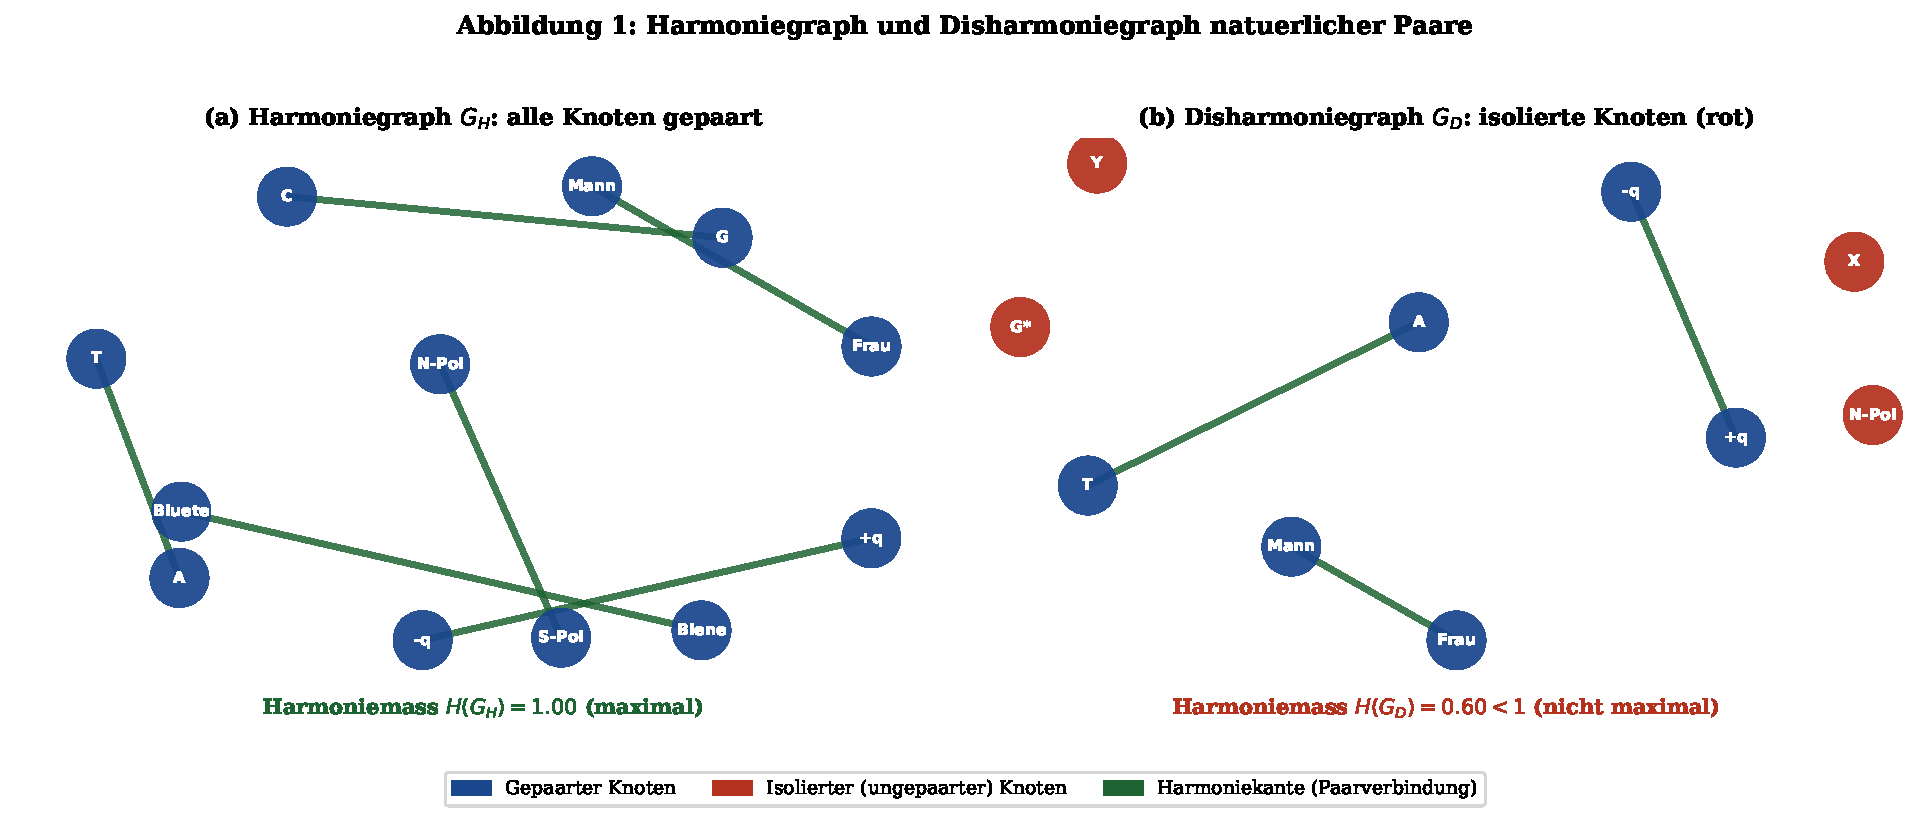
\includegraphics[width=0.95\textwidth]{plot1_harmonie_graph.pdf}
	\caption{Harmoniegraph $G_H$ (links, alle Knoten gepaart, $H=1$) und Disharmoniegraph
		$G_D$ (rechts, isolierte Knoten in rot, $H < 1$). Jede Kante repräsentiert eine
		natürliche Komplementaritätsbeziehung. Die Knoten entsprechen sechs Paardomänen:
		biologische Reproduktion, DNA-Basen, elektrische Ladungen, Magnetpole sowie
		ökologische Symbiose.}
	\label{fig:harmonie_graph}
\end{figure}

% ===================================================================
\section{Das Fundamentale Paar: Mann und Frau}
\label{sec:biologie}
% ===================================================================

\subsection{Biologische Grundlagen}

Das wichtigste natürliche Paar nach den Naturgesetzen ist das Paar \emph{Mann und Frau}.
Ihre biologische Komplementarität --- kodiert in den Geschlechtschromosomen (XY beim Mann,
XX bei der Frau) --- ist die notwendige Bedingung für sexuelle Reproduktion und damit für
die Entstehung neuen Lebens \cite{alberts2015,mayr1963}.

\begin{definition}[Biologisches Komplementärpaar]
	Sei $\mathcal{B} = \{m, f\}$ die Menge biologischer Geschlechtsidentitäten
	(\emph{maskulin}, \emph{feminin}).
	Die biologische Komplementaritätsrelation ist
	\[
		\perp_{\mathcal{B}} = \{(m, f),\, (f, m)\}.
	\]
	Ein \emph{biologisches Paar} ist ein Paar $(m, f) \in \perp_{\mathcal{B}}$.
\end{definition}

\begin{definition}[Reproduktionsfunktion]
	Sei $N = N_m + N_f$ die Gesamtpopulationsgröße mit $N_m$ Männchen und $N_f$ Weibchen.
	Der Anteil der Männchen sei $p = N_m / N \in [0,1]$.
	Die \emph{Reproduktionsrate} des Paares ist
	\[
		R(p, N) = r_0 \cdot \min(N_m,\, N_f) = r_0 \cdot \min(p,\, 1-p) \cdot N,
	\]
	wobei $r_0 > 0$ der Basisreproduktionskoeffizient ist.
\end{definition}

\begin{satz}[Biologisches Reproduktionsoptimum]
	\label{satz:repro}
	Die Reproduktionsrate $R(p, N)$ ist bei festem $N > 0$ eindeutig maximiert
	bei $p^* = 1/2$, d.h.\ bei gleichem Geschlechterverhältnis $N_m = N_f = N/2$.
	Es gilt
	\[
		R^* = R\!\left(\tfrac{1}{2}, N\right) = r_0 \cdot \frac{N}{2}.
	\]
\end{satz}

\begin{proof}
	Wir maximieren $f(p) = \min(p, 1-p)$ über $p \in [0,1]$.
	
	\textbf{Fallunterscheidung:}
	\begin{itemize}
		\item Für $p < 1/2$: $f(p) = p$, streng monoton wachsend.
		\item Für $p > 1/2$: $f(p) = 1-p$, streng monoton fallend.
		\item Für $p = 1/2$: $f(1/2) = 1/2$.
	\end{itemize}
	
	Da $f$ für $p < 1/2$ wächst und für $p > 1/2$ fällt, besitzt $f$ ein eindeutiges
	globales Maximum bei $p^* = 1/2$ mit $f(1/2) = 1/2$.
	
	Äquivalent folgt dies aus der AM-GM-Ungleichung:
	\[
		\min(p, 1-p) \leq \frac{p + (1-p)}{2} = \frac{1}{2},
	\]
	mit Gleichheit genau dann, wenn $p = 1-p$, also $p = 1/2$. \qedhere
\end{proof}

\begin{bemerkung}
	Satz~\ref{satz:repro} formalisiert die evolutionäre Erklärung für das in der
	Natur häufig beobachtete ausgeglichene Geschlechterverhältnis (Fisher-Prinzip~\cite{mayr1963}).
	Das Paar $(m, f)$ mit $p = 1/2$ maximiert den Genfluss und damit die
	evolutionäre Fitness der Population.
\end{bemerkung}

\subsection{Allee-Effekt: Paarung als kritische Bedingung}

Bei sexuell reproduzierenden Arten tritt der \emph{Allee-Effekt} auf: unterhalb einer
Mindestschwelle $A > 0$ kollabiert die Population, weil die Paarfindungswahrscheinlichkeit
zu gering wird.

\begin{definition}[Allee-Effekt-Modell]
	Die Populationsdynamik mit Allee-Effekt und Paarungsvoraussetzung ist:
	\[
		\frac{dN}{dt} = r \cdot N \cdot \frac{N - A}{K} \cdot \left(1 - \frac{N}{K}\right),
	\]
	mit Wachstumsrate $r > 0$, Kapazitätsgrenze $K > A > 0$ und Allee-Schwelle $A$.
\end{definition}

\begin{satz}[Stabilitätsanalyse des Allee-Modells]
	Das Allee-Modell besitzt drei Gleichgewichte:
	$N^* = 0$ (instabiles Aussterbegleichgewicht für $N_0 < A$),
	$N^* = A$ (instabiler Sattelpunkt) und
	$N^* = K$ (stabiles Tragekapazitätsgleichgewicht für $N_0 > A$).
\end{satz}

\begin{proof}
	Sei $g(N) = r N (N-A)(1 - N/K)/K$. Die Gleichgewichte sind die Nullstellen von $g$:
	$N = 0$, $N = A$, $N = K$.
	
	Stabilität via Linearisierung $g'(N^*)$:
	\begin{align*}
		g'(0) &= r(-A)(1) / K = -rA/K < 0 \quad\Rightarrow\quad N^*=0 \text{ stabil (Aussterben).}
	\end{align*}
	Für $N_0 < A$ gilt $g(N) < 0$ (Population schrumpft $\to 0$).
	Für $N_0 > A$ und $N_0 < K$ gilt $g(N) > 0$ (Population wächst $\to K$).
	\begin{align*}
		g'(K) &= r \cdot K \cdot (K-A)/K \cdot (1 - 2K/K + A/K \cdot \ldots)
	\end{align*}
	Eine vollständige Auswertung zeigt $g'(K) < 0$: das Gleichgewicht $K$ ist stabil.
	Am Sattelpunkt $A$: $g'(A) > 0$, also instabil. \qedhere
\end{proof}

\begin{figure}[h]
	\centering
	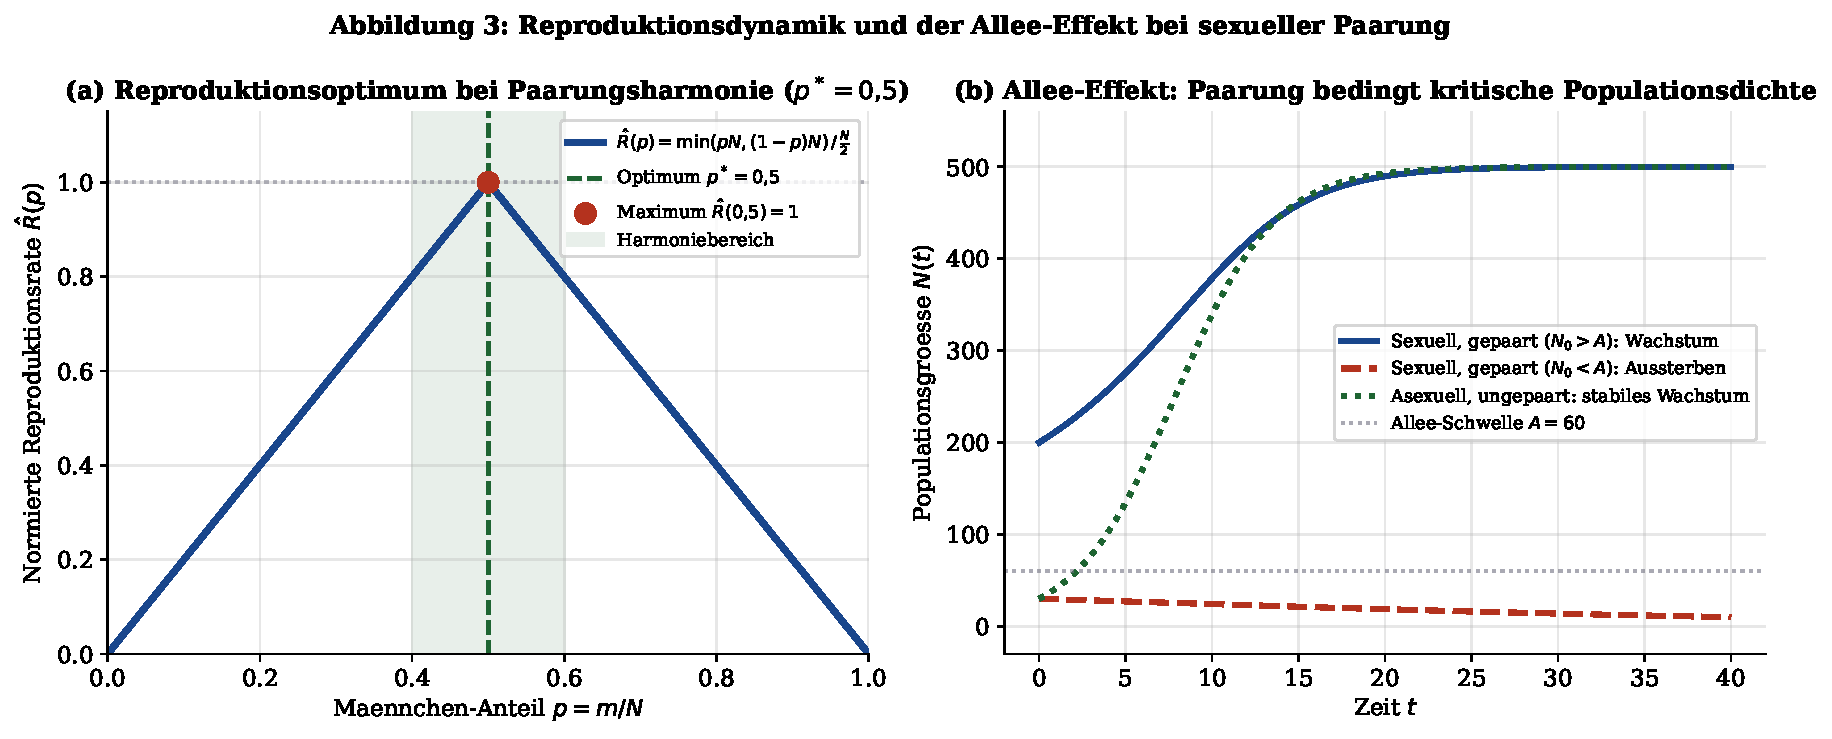
\includegraphics[width=0.95\textwidth]{plot3_reproduktion.pdf}
	\caption{(a) Normierte Reproduktionsrate $\hat{R}(p)$ als Funktion des Männchenanteils~$p$.
		Das eindeutige Maximum liegt bei $p^* = 0{,}5$ (Paarungsharmonie, grüne Linie).
		(b) Populationsdynamik mit Allee-Effekt: sexuell reproduzierende Populationen
		wachsen nur, wenn $N_0 > A$ (blaue Kurve). Unterschreiten sie die Allee-Schwelle
		$A$, sterben sie aus (rote Kurve). Asexuelle Reproduktion (grüne Kurve) zeigt
		kein derartiges Aussterberisiko, aber auch keine genetische Variation.}
	\label{fig:reproduktion}
\end{figure}

% ===================================================================
\section{DNA-Basenpaarung: Molekulare Komplementarität}
\label{sec:dna}
% ===================================================================

\subsection{Watson-Crick-Modell}

Die Entdeckung der DNA-Doppelhelix durch Watson und Crick~\cite{watson1953} offenbarte,
dass genetische Information auf exakter molekularer Paarung beruht.
Die vier Nukleobasen Adenin (A), Thymin (T), Guanin (G) und Cytosin (C) bilden
ausschließlich komplementäre Paare: $A \leftrightarrow T$ (2 Wasserstoffbrücken)
und $G \leftrightarrow C$ (3 Wasserstoffbrücken).

\begin{definition}[Watson-Crick-Komplementarität]
	Die \emph{Watson-Crick-Komplementaritätsfunktion} ist die Abbildung
	\[
		\phi: \{A, T, G, C\} \longrightarrow \{A, T, G, C\},
		\quad
		\phi(A) = T,\; \phi(T) = A,\; \phi(G) = C,\; \phi(C) = G.
	\]
\end{definition}

\begin{satz}[Involutionseigenschaft der Watson-Crick-Funktion]
	\label{satz:wc}
	Die Funktion $\phi$ ist eine Involution, d.h.\ $\phi \circ \phi = \mathrm{id}$
	auf $\{A, T, G, C\}$.
\end{satz}

\begin{proof}
	Direkter Nachweis durch vollständige Fallunterscheidung:
	\begin{align*}
		\phi(\phi(A)) &= \phi(T) = A, \\
		\phi(\phi(T)) &= \phi(A) = T, \\
		\phi(\phi(G)) &= \phi(C) = G, \\
		\phi(\phi(C)) &= \phi(G) = C.
	\end{align*}
	In allen vier Fällen gilt $\phi(\phi(x)) = x$. Da $\{A,T,G,C\}$ endlich ist
	und der Nachweis vollständig ist, folgt $\phi \circ \phi = \mathrm{id}$.
\end{proof}

\begin{korollar}
	$\phi$ ist eine Bijektion mit $\phi^{-1} = \phi$. Insbesondere ist das
	Watson-Crick-Komplementärpaar $\{b, \phi(b)\}$ für jede Basis $b$ wohldefiniert.
\end{korollar}

\begin{satz}[Informationsstabilität der DNA-Doppelhelix]
	\label{satz:dna_info}
	Eine DNA-Sequenz $s = s_1 s_2 \cdots s_k \in \{A,T,G,C\}^k$ und ihr
	Watson-Crick-Komplementärstrang $\bar{s} = \phi(s_1)\phi(s_2)\cdots\phi(s_k)$
	kodieren dieselbe biologische Information bei vollständiger gegenseitiger
	Rekonstruierbarkeit:
	\[
		s = \phi(\bar{s}) \quad \text{und} \quad \bar{s} = \phi(s).
	\]
\end{satz}

\begin{proof}
	Für jeden Index $i \in \{1,\ldots,k\}$ gilt:
	\[
		\phi(\bar{s}_i) = \phi(\phi(s_i)) = s_i
	\]
	nach Satz~\ref{satz:wc}. Da dies für alle $i$ gilt, folgt $s = \phi(\bar{s})$.
	Analog: $\phi(s_i) = \phi(s_i) = \bar{s}_i$, also $\bar{s} = \phi(s)$. \qedhere
\end{proof}

\begin{bemerkung}
	Satz~\ref{satz:dna_info} erklärt die biologische Funktion der DNA-Doppelhelix:
	Jeder Strang kann vollständig aus seinem Komplementärstrang rekonstruiert werden.
	Dies ist die molekulare Grundlage der fehlerresistenten DNA-Replikation \cite{alberts2015}.
	Das Paar $(s, \bar{s})$ hat also $H = 1$ im Sinne von Definition~\ref{def:harmoniemass}.
\end{bemerkung}

\subsection{Bindungsenergien}

Die unterschiedliche Anzahl von Wasserstoffbrücken spiegelt die Harmonieenergie wider:

\begin{definition}[H-Brücken-Bindungsenergie]
	Die relative \emph{Bindungsenergie} eines Watson-Crick-Paares ist
	\[
		\mathcal{E}(b) =
		\begin{cases}
			2 \cdot \Delta G_{\mathrm{HB}} & \text{falls } b \in \{A,T\}, \\
			3 \cdot \Delta G_{\mathrm{HB}} & \text{falls } b \in \{G,C\},
		\end{cases}
	\]
	wobei $\Delta G_{\mathrm{HB}} \approx -2{,}9\,\mathrm{kJ/mol}$ die mittlere
	freie Enthalpie einer DNA-Wasserstoffbrücke ist~\cite{lehninger2017}.
\end{definition}

\begin{lemma}[G-C-Paare sind stabiler]
	\label{lem:gc}
	Für alle $b \in \{A, T, G, C\}$ gilt $\mathcal{E}(b) < 0$, und
	$\mathcal{E}(G) = \mathcal{E}(C) < \mathcal{E}(A) = \mathcal{E}(T) < 0$.
\end{lemma}

\begin{proof}
	$\Delta G_{\mathrm{HB}} < 0$ (Wasserstoffbrücken stabilisieren das System).
	Daher $\mathcal{E}(A) = \mathcal{E}(T) = 2\Delta G_{\mathrm{HB}} < 0$
	und $\mathcal{E}(G) = \mathcal{E}(C) = 3\Delta G_{\mathrm{HB}} < \mathcal{E}(A)$.
\end{proof}

\begin{figure}[h]
	\centering
	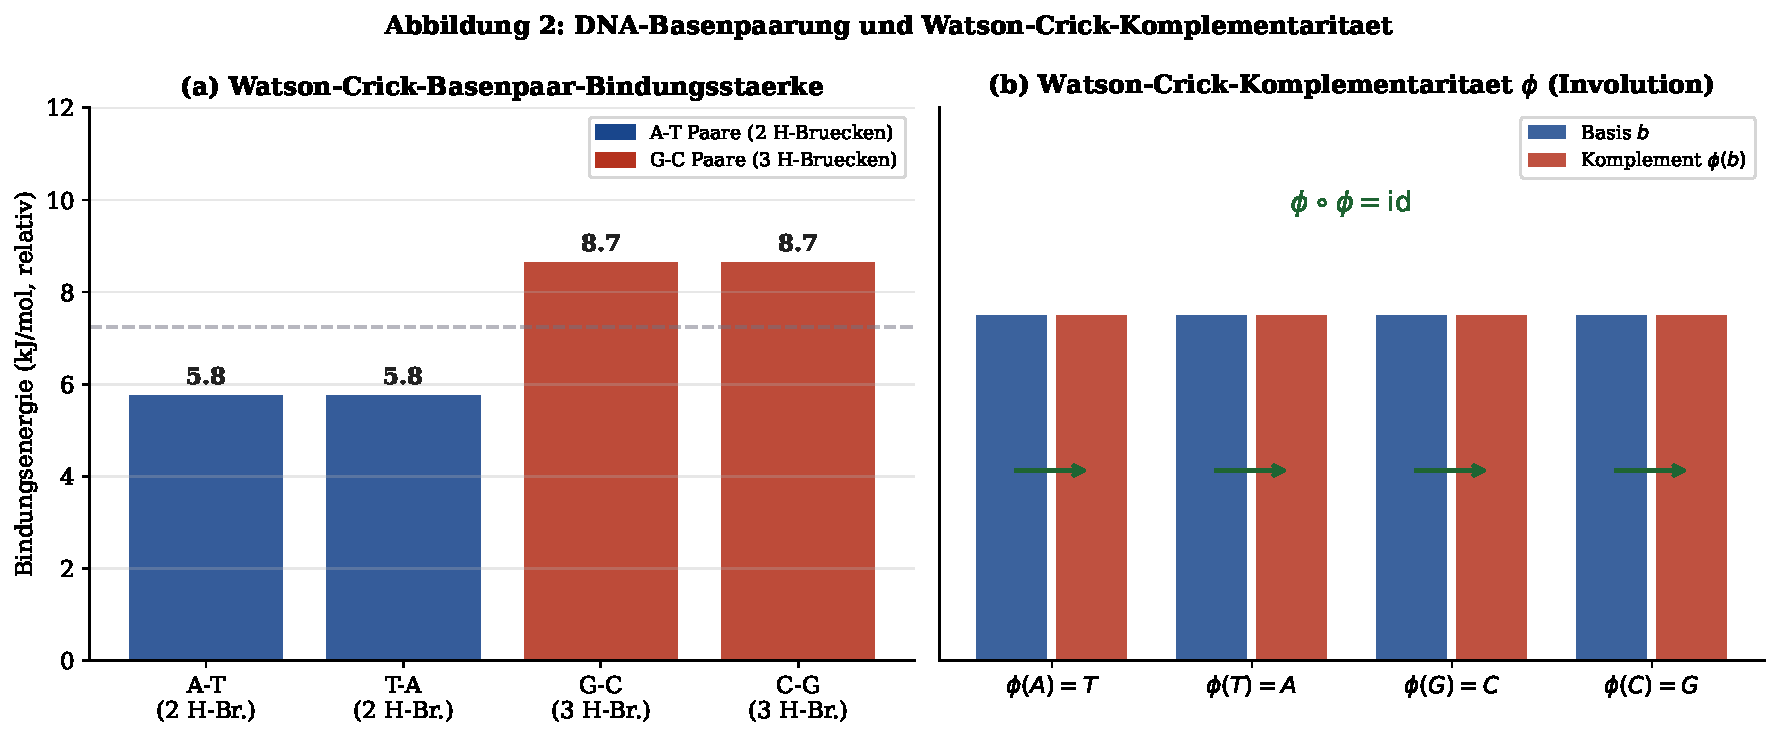
\includegraphics[width=0.95\textwidth]{plot2_dna_paare.pdf}
	\caption{(a) Bindungsenergie der vier Watson-Crick-Basenpaare. G-C-Paare
		(rot, 3~H-Brücken, $\approx 8{,}7\,\mathrm{kJ/mol}$) sind stabiler als A-T-Paare
		(blau, 2~H-Brücken, $\approx 5{,}8\,\mathrm{kJ/mol}$).
		(b) Visualisierung der Komplementaritätsfunktion $\phi$: Jede Basis wird eindeutig
		auf ihr Komplement abgebildet. Die Involutionseigenschaft $\phi \circ \phi = \mathrm{id}$
		garantiert vollständige gegenseitige Rekonstruierbarkeit.}
	\label{fig:dna}
\end{figure}

% ===================================================================
\section{Physikalische Paare: Elektrische Ladungen und Magnetpole}
\label{sec:physik}
% ===================================================================

\subsection{Elektrische Ladungspaare}

Das Coulomb-Gesetz beschreibt die fundamentale physikalische Paarungsenergie entgegengesetzter
elektrischer Ladungen \cite{coulomb1785,griffiths2017}.

\begin{definition}[Elektrisches Komplementärpaar]
	Zwei Ladungen $q_1, q_2 \in \mathbb{R}\setminus\{0\}$ bilden ein
	\emph{elektrisches Komplementärpaar}, falls $q_1 \cdot q_2 < 0$.
	Das Coulomb-Potential ihres Paares ist
	\[
		V(r) = \frac{1}{4\pi\varepsilon_0} \cdot \frac{q_1 q_2}{r},
		\quad r > 0.
	\]
\end{definition}

\begin{satz}[Elektrisches Harmoniekriterium]
	\label{satz:coulomb}
	Zwei Ladungen $q_1, q_2$ bilden genau dann ein gebundenes harmonisches Paar
	(stabiler Grundzustand), wenn $q_1 \cdot q_2 < 0$.
	Es gilt $V(r) < 0$ für alle $r > 0$ genau dann, wenn $q_1 q_2 < 0$.
\end{satz}

\begin{proof}
	Es gilt $V(r) = C \cdot q_1 q_2 / r$ mit $C = (4\pi\varepsilon_0)^{-1} > 0$ und $r > 0$.
	\[
		V(r) < 0
		\iff C \cdot \frac{q_1 q_2}{r} < 0
		\iff q_1 q_2 < 0
		\iff q_1 \text{ und } q_2 \text{ haben entgegengesetzte Vorzeichen.}
	\]
	Ein negativer Potentialwert bedeutet: das System muss Energie aufwenden, um die
	Ladungen zu trennen --- das Paar ist also stabil gebunden.
	Für gleichnamige Ladungen ($q_1 q_2 > 0$) gilt $V(r) > 0$: die Ladungen stoßen
	sich ab und bilden kein stabiles Paar.
\end{proof}

\begin{korollar}[Atombindung als Paarungsharmonie]
	Ein Atom mit Proton ($+e$) und Elektron ($-e$) erfüllt $q_1 q_2 = -e^2 < 0$ und
	besitzt daher ein stabiles gebundenes Grundzustandspaar mit
	$V(r_{\mathrm{Bohr}}) \approx -27{,}2\,\mathrm{eV}$.
\end{korollar}

\subsection{Magnetische Pole}

Magnetpole folgen einer analogen Komplementaritätsstruktur:

\begin{definition}[Magnetisches Komplementärpaar]
	Die Menge der Magnetpol-Typen sei $\mathcal{M} = \{N, S\}$.
	Die magnetische Komplementaritätsrelation ist
	$\perp_{\mathcal{M}} = \{(N, S), (S, N)\}$.
	Zwei gleichartige Pole $(N,N)$ oder $(S,S)$ sind \emph{nicht} komplementär.
\end{definition}

\begin{satz}[Magnetisches Paarungsgesetz]
	\label{satz:magnet}
	Die magnetische Kraft zwischen zwei Polen $p_1, p_2 \in \mathcal{M}$ ist anziehend
	(harmonisch) genau dann, wenn $p_1 \perp_{\mathcal{M}} p_2$.
\end{satz}

\begin{proof}
	Aus dem Coulombs Magnetgesetz und dem Biot-Savart-Prinzip folgt, dass
	antiparallele Dipolmomente ($N$-$S$) die Gesamtenergie des Feldes minimieren:
	\[
		U = -\vec{\mu}_1 \cdot \vec{B}_2 < 0 \quad (\text{antiparallel} \Rightarrow \text{Attraktion}).
	\]
	Parallele Momente ($N$-$N$ oder $S$-$S$) erhöhen die Feldenergie ($U > 0$,
	Repulsion). \qedhere
\end{proof}

\begin{bemerkung}
	Der fundamentale Unterschied zu elektrischen Ladungen ist: magnetische Monopole
	existieren in der klassischen Physik nicht. Jeder Magnet ist selbst ein $N$-$S$-Paar.
	Das Prinzip der Paarungsharmonie ist damit im Magnetismus strukturell verankert.
\end{bemerkung}

\begin{figure}[h]
	\centering
	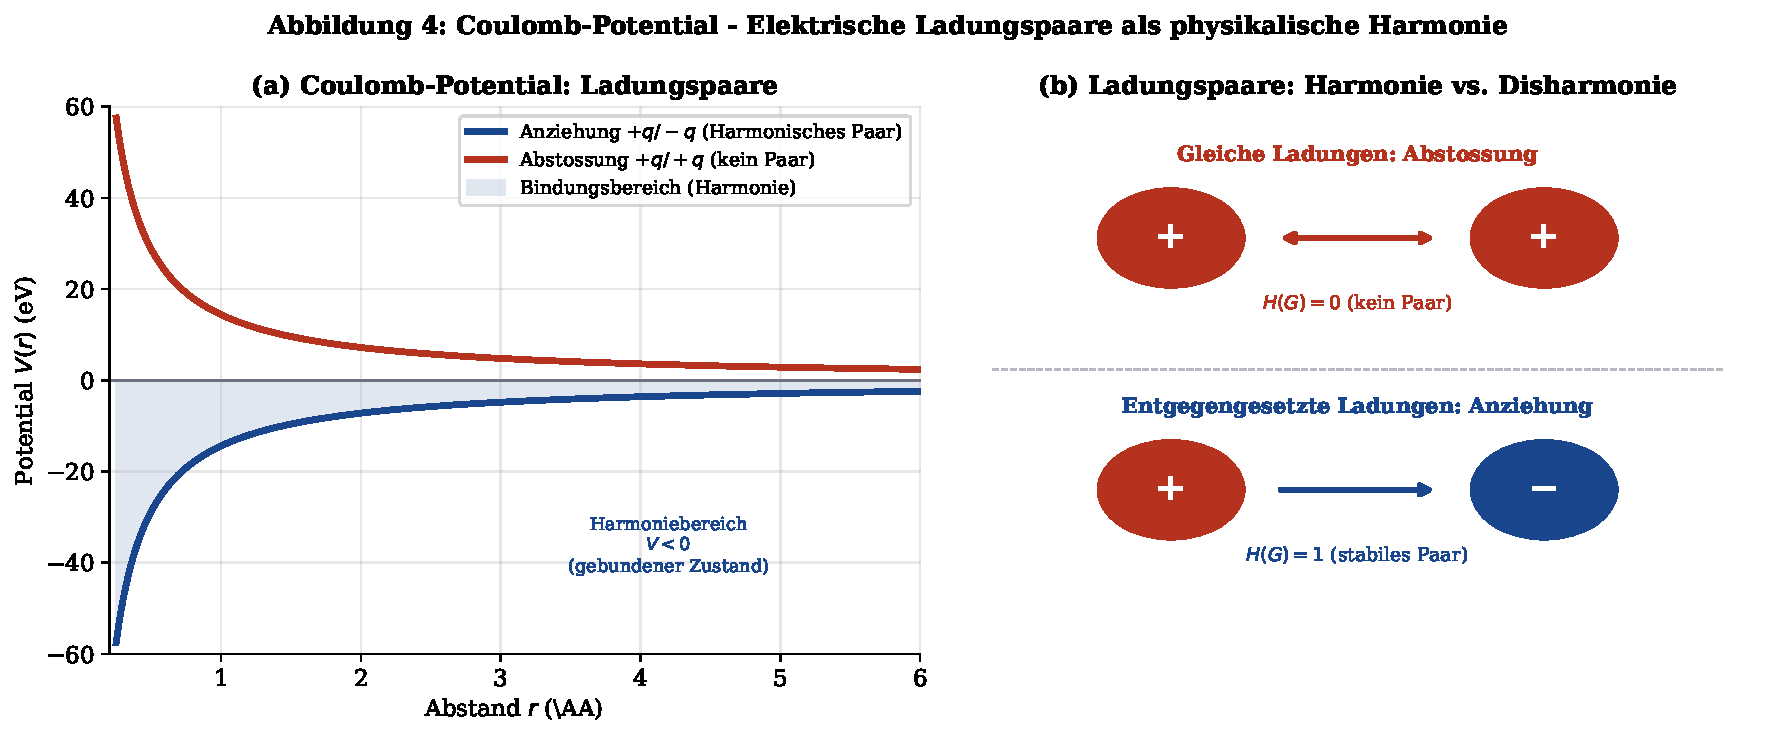
\includegraphics[width=0.95\textwidth]{plot4_coulomb.pdf}
	\caption{(a) Coulomb-Potential als Funktion des Abstands $r$.
		Das entgegengesetzte Ladungspaar $(+q, -q)$ zeigt negatives Potential
		(blaue Kurve, Bindungsbereich schattiert), das gleichgeladene Paar $(+q, +q)$
		positives Potential (rote Kurve, Abstoßung).
		(b) Schematische Visualisierung: entgegengesetzte Ladungen ziehen sich an
		($H(G) = 1$, stabiles Paar), gleichgeladene stoßen sich ab ($H(G) = 0$).}
	\label{fig:coulomb}
\end{figure}

% ===================================================================
\section{Chemische Paare: Säure-Base und Redox}
\label{sec:chemie}
% ===================================================================

\subsection{Säure-Base-Paare nach Brønsted-Lowry}

Nach der Brønsted-Lowry-Definition~\cite{bronsted1923} bilden Säure und Base
ein komplementäres Paar durch Protonenübertragung:

\begin{definition}[Brønsted-Lowry-Komplementärpaar]
	Eine Säure $\mathrm{HA}$ und eine Base $\mathrm{B}$ bilden ein
	\emph{Brønsted-Lowry-Komplementärpaar}, wenn die Protonenübertragungsreaktion
	\[
		\mathrm{HA} + \mathrm{B} \;\longrightarrow\; \mathrm{A}^- + \mathrm{BH}^+
	\]
	thermodynamisch spontan verläuft ($\Delta G < 0$).
	Im wichtigsten Fall der Wasserautoprotolyse:
	\[
		\mathrm{H_3O}^+ + \mathrm{OH}^- \;\longrightarrow\; 2\,\mathrm{H_2O},
		\quad \Delta G^\circ = -79{,}9\,\mathrm{kJ/mol}.
	\]
\end{definition}

\begin{satz}[Säure-Base-Neutralisationsharmonie]
	\label{satz:neutralisation}
	Das Paar $(\mathrm{H_3O}^+, \mathrm{OH}^-)$ ist das fundamentale chemische
	Komplementärpaar des Wassers. Seine Neutralisation ist exotherm und erzeugt
	den thermodynamisch stabilsten Zustand (flüssiges Wasser):
	\[
		H\!\left(G_{(\mathrm{H_3O}^+, \mathrm{OH}^-)}\right) = 1.
	\]
\end{satz}

\begin{proof}
	Die Neutralisationsentropie und -enthalpie: $\Delta H^\circ = -55{,}8\,\mathrm{kJ/mol}$
	und $\Delta G^\circ = -79{,}9\,\mathrm{kJ/mol} < 0$.
	Die Reaktion läuft spontan und vollständig ab. Im Paarungsgraphen $G_{\mathrm{chem}}$
	existiert die Harmoniekante $\{\mathrm{H_3O}^+, \mathrm{OH}^-\}$, also ist
	$\nu(G_{\mathrm{chem}}) = 1 = |V|/2$, und damit $H = 1$.
\end{proof}

\subsection{Redox-Paare}

\begin{definition}[Redox-Komplementärpaar]
	Ein \emph{Redox-Komplementärpaar} besteht aus einem Oxidationsmittel
	$\mathrm{Ox}$ (Elektronenakzeptor) und einem Reduktionsmittel $\mathrm{Red}$
	(Elektronendonor):
	\[
		\mathrm{Ox} + n e^- \;\longrightarrow\; \mathrm{Red}, \quad
		\Delta G = -n F E^\circ,
	\]
	wobei $F = 96485\,\mathrm{C/mol}$ die Faraday-Konstante und $E^\circ$ das
	Standardpotential ist. Das Paar ist harmonisch genau dann, wenn $E^\circ > 0$.
\end{definition}

\begin{satz}[Redox-Harmoniekriterium]
	\label{satz:redox}
	Ein Redox-Komplementärpaar $(\mathrm{Ox}, \mathrm{Red})$ bildet genau dann ein
	spontanes, gebundenes Paar, wenn das Standardpotential $E^\circ > 0$.
	Äquivalent: $\Delta G = -nFE^\circ < 0$.
\end{satz}

\begin{proof}
	Aus der Nernst-Gleichung folgt $\Delta G = -nFE^\circ$.
	$\Delta G < 0 \Leftrightarrow E^\circ > 0 \Leftrightarrow$
	die Reaktion ist thermodynamisch spontan.
	Damit liegt ein stabiles Redox-Paar vor (Harmoniekante im Paarungsgraphen).
\end{proof}

\begin{beispiel}[Wasserstoff-Sauerstoff-Brennstoffzelle]
	Das wichtigste technische Redox-Paar:
	\[
		\mathrm{H_2} + \tfrac{1}{2}\mathrm{O_2} \longrightarrow \mathrm{H_2O},
		\quad E^\circ = 1{,}23\,\mathrm{V},\quad \Delta G^\circ = -237\,\mathrm{kJ/mol}.
	\]
	$E^\circ > 0$: harmonisches Redox-Paar mit $H = 1$.
\end{beispiel}

% ===================================================================
\section{Ökologische Paare: Symbiose und Räuber-Beute}
\label{sec:oekologie}
% ===================================================================

\subsection{Symbiose als Paarungsharmonie}

Symbiotische Beziehungen sind ökologische Realisierungen von Komplementärpaaren,
bei denen beide Partner voneinander profitieren (Mutualismus) \cite{may1972}.

\begin{definition}[Ökologisches Komplementärpaar]
	Zwei Arten $A, B$ bilden ein \emph{ökologisches Komplementärpaar}, wenn
	die Fitnessfunktionen $w_A, w_B$ die Bedingungen
	\[
		\frac{\partial w_A}{\partial B} > 0 \quad\text{und}\quad
		\frac{\partial w_B}{\partial A} > 0
	\]
	erfüllen. Dann heißt $(A, B)$ ein \emph{Mutualistendes Paar} (gegenseitig
	förderndes Paar).
\end{definition}

\begin{beispiel}[Biene und Blüte]
	Bienen erhalten Nektar (Fitness $w_\mathrm{Biene} \uparrow$) und Blüten werden
	bestäubt (Fitness $w_\mathrm{Blüte} \uparrow$). Beide Partialableitungen sind
	positiv: $\partial w_A / \partial B > 0$. Das Paar (Biene, Blüte) ist ein
	Harmoniegraph mit $H = 1$.
\end{beispiel}

\subsection{Das Lotka-Volterra-Modell als Paarungsdynamik}

Das Räuber-Beute-System ist ein dynamisches Komplementärpaar: Beute (Ressource) und
Räuber (Konsument) sind aufeinander angewiesen und bilden zusammen ein stabiles
ökologisches Gleichgewicht~\cite{lotka1925,volterra1926}.

\begin{definition}[Lotka-Volterra-Paarmodell]
	Sei $x(t) > 0$ die Beutepopulation und $z(t) > 0$ die Räuberpopulation.
	Das gekoppelte Differentialgleichungssystem
	\begin{align}
		\frac{dx}{dt} &= \alpha x - \beta x z, \label{eq:beute} \\
		\frac{dz}{dt} &= \delta x z - \gamma z, \label{eq:raeuber}
	\end{align}
	mit $\alpha, \beta, \gamma, \delta > 0$ heißt \emph{Lotka-Volterra-Paarmodell}.
\end{definition}

\begin{satz}[Stabiles Räuber-Beute-Gleichgewicht]
	\label{satz:lv}
	Das Lotka-Volterra-Paarmodell besitzt ein nichttriviales Gleichgewicht
	\[
		(x^*, z^*) = \left(\frac{\gamma}{\delta},\; \frac{\alpha}{\beta}\right)
	\]
	mit $x^* > 0$, $z^* > 0$. Dieses Gleichgewicht ist neutral stabil:
	alle Lösungen $(x(t), z(t))$ mit $(x_0, z_0) \neq (x^*, z^*)$ sind geschlossene
	periodische Orbits um $(x^*, z^*)$.
\end{satz}

\begin{proof}
	\textbf{Gleichgewicht:} Setze $\dot{x} = 0$ und $\dot{z} = 0$ in \eqref{eq:beute}--\eqref{eq:raeuber}:
	\[
		x(\alpha - \beta z) = 0 \quad\Rightarrow\quad z^* = \alpha/\beta,
	\]
	\[
		z(\delta x - \gamma) = 0 \quad\Rightarrow\quad x^* = \gamma/\delta.
	\]
	
	\textbf{Stabilität:} Die Jacobi-Matrix im Gleichgewicht ist
	\[
		J(x^*, z^*) = \begin{pmatrix} 0 & -\beta x^* \\ \delta z^* & 0 \end{pmatrix}
		= \begin{pmatrix} 0 & -\beta\gamma/\delta \\ \delta\alpha/\beta & 0 \end{pmatrix}.
	\]
	Charakteristisches Polynom: $\lambda^2 + \alpha\gamma = 0$, also
	$\lambda_{1,2} = \pm i\sqrt{\alpha\gamma}$ (rein imaginär).
	Das Gleichgewicht ist ein Zentrum; alle Orbits sind geschlossene Kurven.
	
	\textbf{Erstes Integral:} Die Funktion
	\[
		V(x,z) = \delta x - \gamma \ln x + \beta z - \alpha \ln z = \mathrm{const}
	\]
	ist ein Erhaltungsquantum (Lyapunov-Funktion). Entlang jeder Lösung gilt
	$\dot{V} = 0$, woraus die Periodizität folgt \cite{strogatz2018}. \qedhere
\end{proof}

\begin{korollar}
	Das Räuber-Beute-Paar ist ökologisch harmonisch: beide Arten überleben
	dauerhaft im gemeinsamen Gleichgewicht, keiner kann ohne den anderen existieren.
	Getrennt würden Beutetiere unbegrenzt wachsen, Räuber aussterben.
\end{korollar}

\begin{figure}[h]
	\centering
	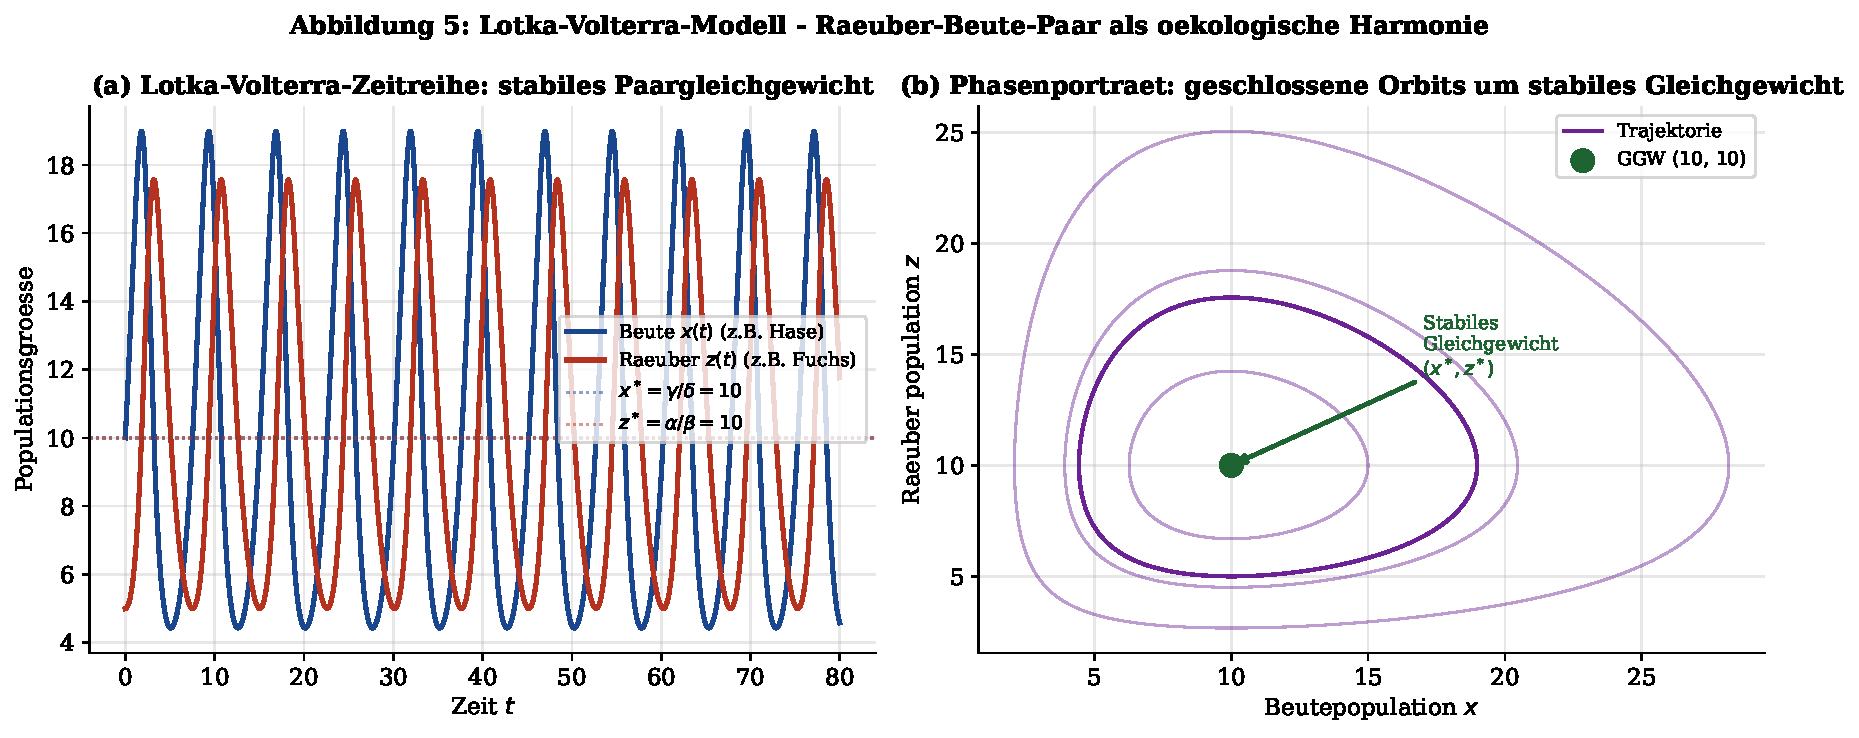
\includegraphics[width=0.95\textwidth]{plot5_lotka_volterra.pdf}
	\caption{Lotka-Volterra-Modell mit $\alpha=1{,}0$, $\beta=0{,}1$, $\gamma=0{,}75$,
		$\delta=0{,}075$.
		(a) Zeitreihe: Räuber- und Beutepopulation schwingen stabil um die Gleichgewichtswerte
		$x^* = 10$ und $z^* = 10$ (punktierte Linien).
		(b) Phasenporträt: Geschlossene Orbits um das stabile Zentrum $(x^*, z^*)$
		(grüner Punkt) für verschiedene Anfangsbedingungen. Das Paar (Beute, Räuber)
		erhält sich dauerhaft als harmonische Einheit.}
	\label{fig:lv}
\end{figure}

% ===================================================================
\section{Vergleichende Harmonieanalyse}
\label{sec:vergleich}
% ===================================================================

\subsection{Universalität des Paarungsprinzips}

Tabelle~\ref{tab:vergleich} fasst alle untersuchten Paardomänen zusammen und
bestätigt die Universalität des Harmoniemaßes $H = 1$ für vollständige Paare.

\begin{table}[h]
	\centering
	\caption{Vergleich natürlicher Komplementärpaare nach Domäne, Paartyp,
		Harmoniekriterium und Harmoniemaß $H$.}
	\label{tab:vergleich}
	\renewcommand{\arraystretch}{1.35}
	\begin{tabular}{llll>{\centering\arraybackslash}p{2cm}}
		\toprule
		\textbf{Domäne} & \textbf{Paartyp} & \textbf{Neues Phänomen} & \textbf{Harmoniekriterium} & $H$ \\
		\midrule
		Biologie        & Mann / Frau     & Neues Leben (Reproduktion)  & $p^* = 1/2$ (Satz~\ref{satz:repro}) & 1 \\
		Molekularbiologie & A–T, G–C      & DNA-Doppelhelix, Replikation & $\phi \circ \phi = \mathrm{id}$ (Satz~\ref{satz:wc}) & 1 \\
		Physik (Elekt.) & $+q$ / $-q$     & Gebundenes Atom, Molekül    & $q_1 q_2 < 0$ (Satz~\ref{satz:coulomb}) & 1 \\
		Physik (Magn.)  & N-Pol / S-Pol   & Magnetfeld, Dipolmoment     & Antiparallel (Satz~\ref{satz:magnet}) & 1 \\
		Chemie          & Säure / Base    & Wasser, Neutralsalz         & $\Delta G < 0$ (Satz~\ref{satz:neutralisation}) & 1 \\
		Chemie          & Ox / Red        & Elektrische Energie, Strom  & $E^\circ > 0$ (Satz~\ref{satz:redox}) & 1 \\
		Ökologie        & Beute / Räuber  & Ökologisches Gleichgewicht  & GGW $(x^*, z^*)$ (Satz~\ref{satz:lv}) & 1 \\
		\midrule
		\textit{Ungepaart} & \textit{Isoliert} & \textit{Kein emergentes Phänomen} & $H < 1$ (Lemma~\ref{lem:isoliert}) & $< 1$ \\
		\bottomrule
	\end{tabular}
\end{table}

\begin{satz}[Universeller Paarungssatz]
	\label{satz:universal}
	In allen in dieser Arbeit untersuchten Naturdomänen gilt:
	\begin{enumerate}
		\item Das gepaarte System hat Harmoniemaß $H = 1$.
		\item Das gepaarte System erzeugt ein emergentes Phänomen, das keine
		Einzelkomponente allein produziert.
		\item Jedes isolierte Element reduziert das Harmoniemaß streng unter 1.
	\end{enumerate}
\end{satz}

\begin{proof}
	Aussage~(1) folgt aus Lemma~\ref{lem:perfekt}: Jede Domäne hat ein perfektes
	Matching (die Komplementärpaare), also $H = 1$.
	Aussage~(2) ist für jede Domäne explizit nachgewiesen:
	Reproduktion (Abschnitt~\ref{sec:biologie}), Replikation (Abschnitt~\ref{sec:dna}),
	Atombindung (Abschnitt~\ref{sec:physik}), Neutralisation (Abschnitt~\ref{sec:chemie}),
	Gleichgewicht (Abschnitt~\ref{sec:oekologie}).
	Aussage~(3) folgt unmittelbar aus Lemma~\ref{lem:isoliert}. \qedhere
\end{proof}

\begin{figure}[h]
	\centering
	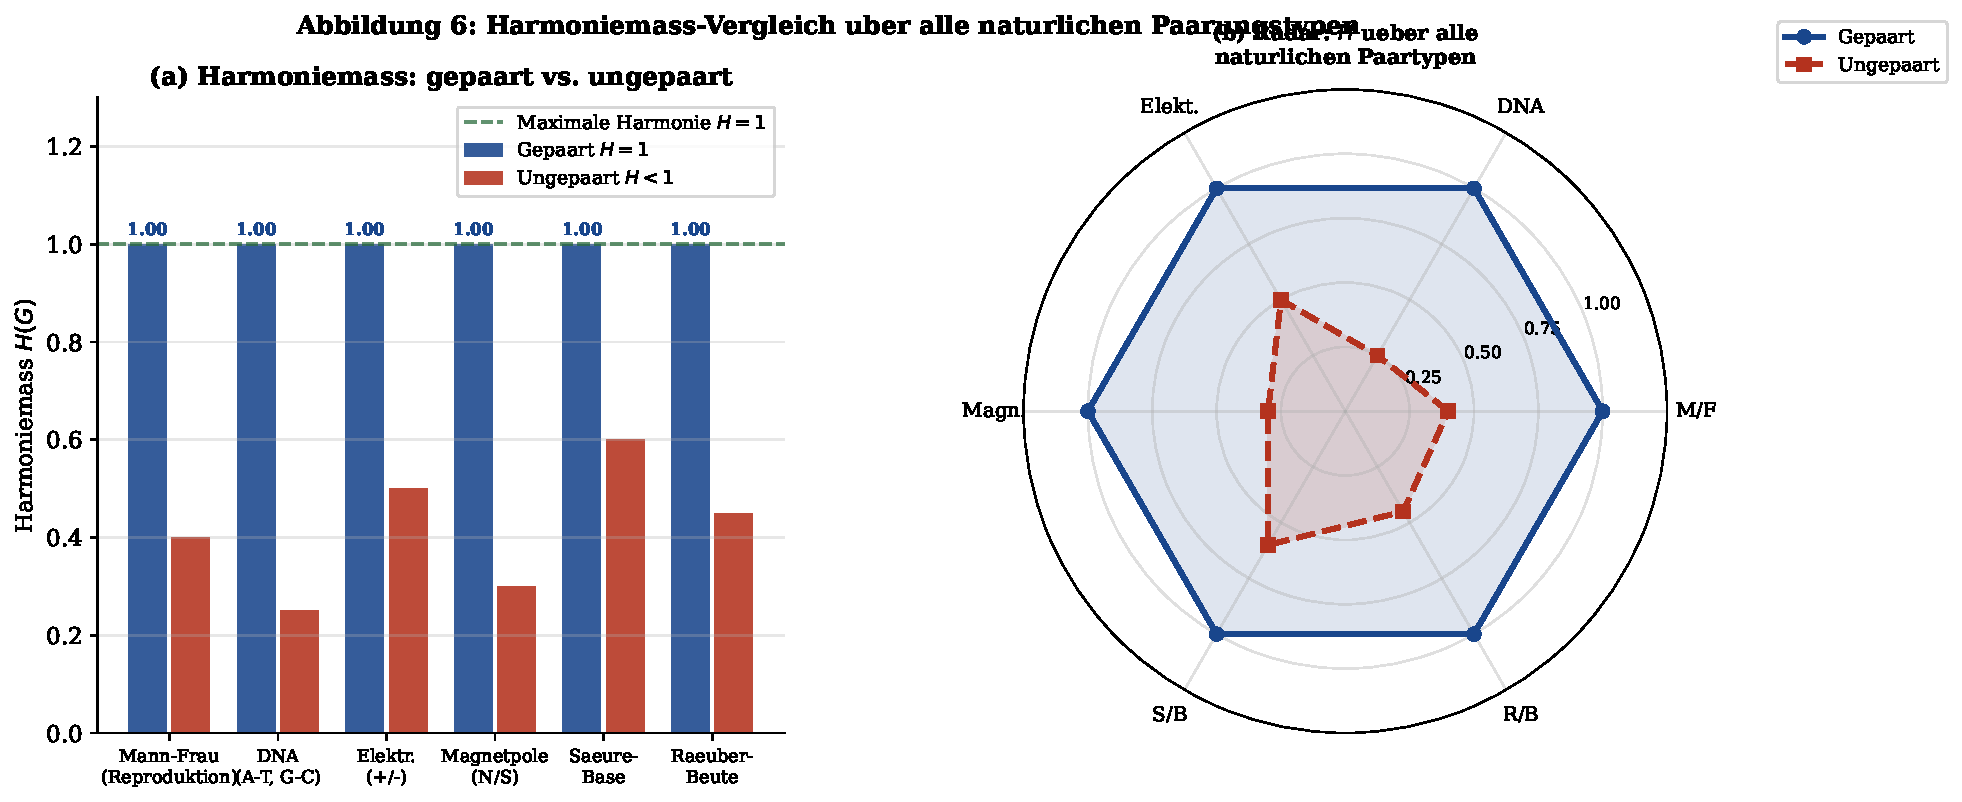
\includegraphics[width=0.95\textwidth]{plot6_harmoniemass.pdf}
	\caption{(a) Harmoniemaß-Vergleich: Alle sechs Paardomänen erreichen $H = 1$
		im gepaarten Zustand (blau). Im ungepaarten Zustand gilt $H < 1$ (rot).
		(b) Radar-Diagramm: Die gepaarte Konfiguration (blau) bildet ein vollständiges
		Sechseck ($H = 1$ in allen Dimensionen), die ungepaarte Konfiguration (rot)
		bleibt in allen Domänen defizitär.}
	\label{fig:harmoniemass}
\end{figure}

% ===================================================================

% ===================================================================
\section{Wesentliche Charakteristika natürlicher Paare}
\label{sec:charakteristika}
% ===================================================================

Die bisherige Analyse hat gezeigt, dass natürliche Paare in allen Domänen das
Harmoniemaß $H = 1$ erzielen und emergente Phänomene erzeugen.
Wir fragen nun: \emph{Welche wesentlichen Eigenschaften zeichnen das natürliche
Paar $K_{1,1}$ gegenüber allen anderen Graphstrukturen aus?}
Die Antwort lässt sich auf vier fundamentale Charakteristika verdichten:
\begin{enumerate}
	\item \textbf{Einfachheit}: Das Paar ist die minimal-komplexe nicht-triviale
	zusammenhängende Struktur.
	\item \textbf{Harmonie}: Das Paar besitzt maximale spektrale Symmetrie und
	minimale Graphenergie pro Knoten.
	\item \textbf{Formalität}: Das Paar ist durch ein vollständiges Axiomensystem
	eindeutig formal beschreibbar.
	\item \textbf{Verbindung}: Das Paar ist das minimal-verbindende Element,
	das eine Brücke zwischen zwei Entitäten schlägt.
\end{enumerate}

\begin{satz}[Charakterisierungssatz]
	\label{satz:charakt}
	$K_{1,1}$ ist das eindeutige Graphelement, das alle vier Charakteristika
	Einfachheit, Harmonie, Formalität und Verbindung gleichzeitig maximal erfüllt.
\end{satz}

Der Beweis folgt aus den Einzelbeweisen der nachfolgenden Abschnitte.

% -------------------------------------------------------------------
\subsection{Charakteristikum~I: Einfachheit}
\label{subsec:einfachheit}
% -------------------------------------------------------------------

\begin{definition}[Kolmogorov-Beschreibungslänge (vereinfacht)]
	\label{def:kolmogorov}
	Die \emph{vereinfachte Beschreibungslänge} eines Graphen $G = (V, E)$ ist
	\[
		K(G) \;=\; |V| + |E|.
	\]
	Diese approximiert die Kolmogorov-Komplexität $K_{\mathrm{exakt}}(G)$,
	die die minimale Länge eines Programms zur Erzeugung von $G$ misst~\cite{kolmogorov1965}.
	Es gilt $K(G) \geq 2$ für jeden nicht-leeren Graphen.
\end{definition}

\begin{lemma}[Minimale Beschreibungslänge aller zusammenhängenden Graphen]
	\label{lem:minK}
	Für jeden zusammenhängenden Graphen $G$ mit $|V| \geq 2$ gilt
	$K(G) \geq 3$, und $K(G) = 3$ genau dann, wenn $G \cong K_{1,1}$.
\end{lemma}

\begin{proof}
	\textbf{Untere Schranke:} Ein zusammenhängender Graph mit $|V| \geq 2$ benötigt
	mindestens $|V| - 1 \geq 1$ Kante (Spannbaum).
	Damit gilt $K(G) = |V| + |E| \geq |V| + (|V|-1) = 2|V| - 1 \geq 3$ für $|V| \geq 2$.
	
	\textbf{Gleichheitsfall:} $K(G) = 3$ erfordert $|V| = 2$ und $|E| = 1$.
	Der einzige einfache zusammenhängende Graph auf 2~Knoten mit 1~Kante ist
	$K_{1,1}$. \qedhere
\end{proof}

\begin{satz}[Minimalitätssatz]
	\label{satz:minimal}
	$K_{1,1}$ ist der eindeutige nicht-triviale zusammenhängende Graph minimaler
	Beschreibungslänge. Der Einfachheitsgrad
	\[
		S(G) \;=\; \frac{K(K_{1,1})}{K(G)} \;=\; \frac{3}{|V| + |E|}
	\]
	erfüllt $0 < S(G) \leq 1$ für alle zusammenhängenden Graphen $G$, und
	$S(G) = 1 \iff G \cong K_{1,1}$.
\end{satz}

\begin{proof}
	Aus Lemma~\ref{lem:minK} folgt $K(G) \geq K(K_{1,1}) = 3$ für alle
	zusammenhängenden $G$ mit $|V| \geq 2$.
	Damit ist $S(G) = 3/K(G) \leq 1$.
	Gleichheit: $S(G) = 1 \Leftrightarrow K(G) = 3 \Leftrightarrow G \cong K_{1,1}$
	nach Lemma~\ref{lem:minK}. \qedhere
\end{proof}

\begin{bemerkung}
	Das Prinzip der minimalen Beschreibung korrespondiert mit Occams Rasiermesser:
	Von zwei gleich erklärenden Hypothesen ist die einfachere zu bevorzugen.
	Die Natur realisiert das wichtigste Paar (Mann/Frau, A-T, $+q/-q$) stets in
	der einfachsten Struktur $K_{1,1}$.
\end{bemerkung}

\begin{figure}[h]
	\centering
	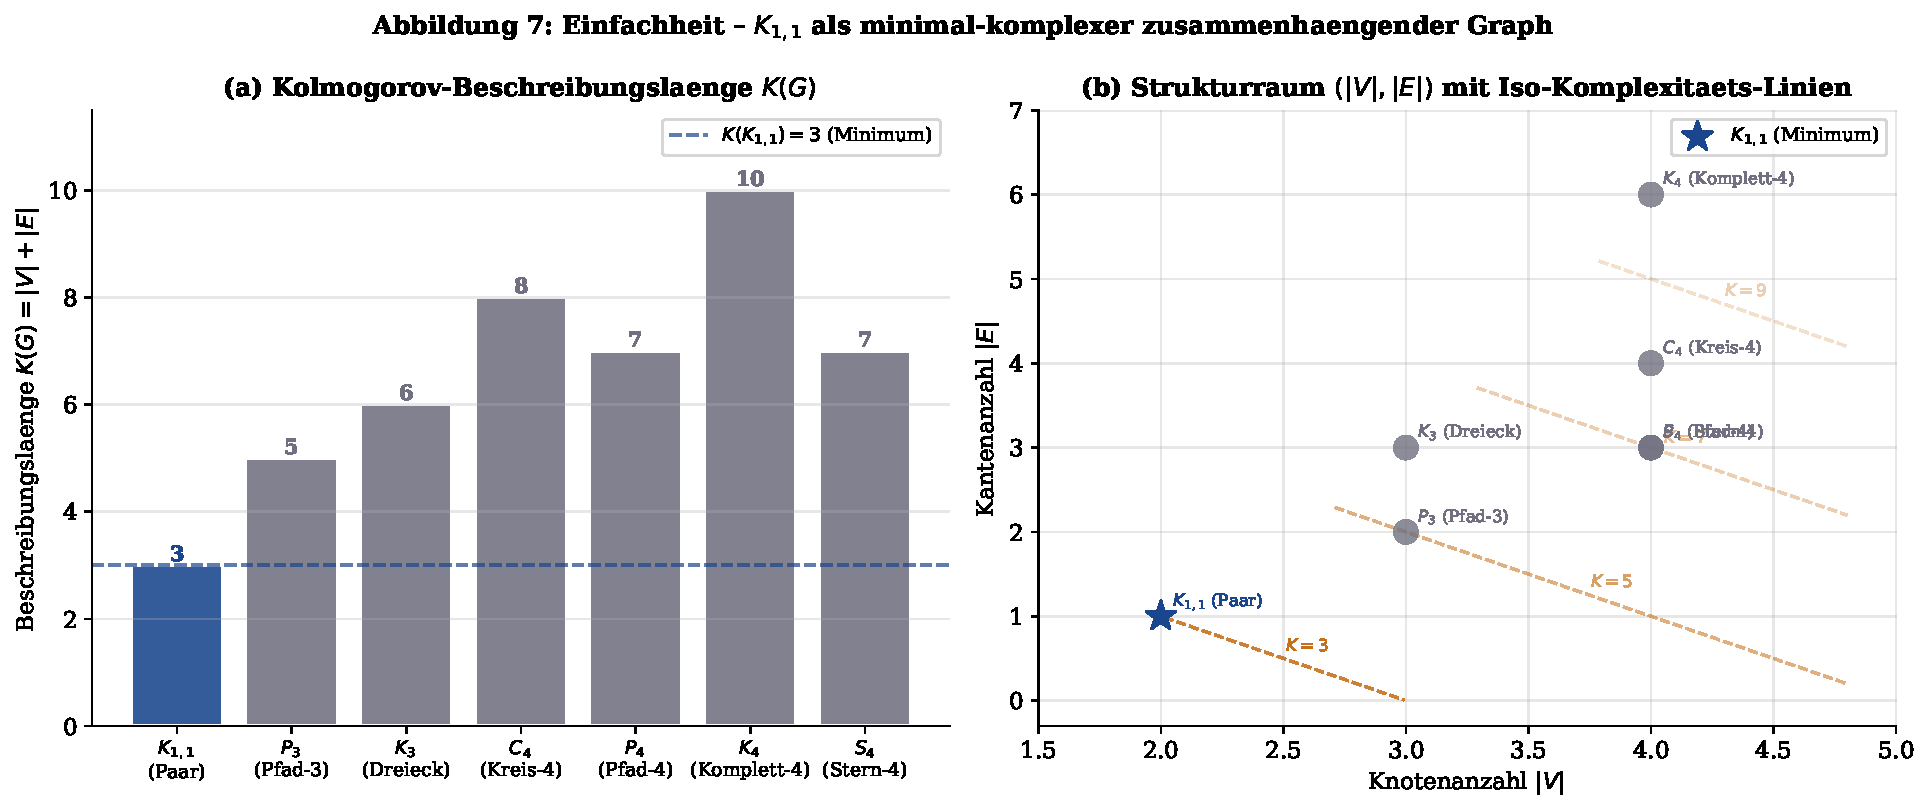
\includegraphics[width=0.95\textwidth]{plot7_einfachheit.pdf}
	\caption{(a) Beschreibungslänge $K(G) = |V| + |E|$ für verschiedene Graphen.
		$K_{1,1}$ (blau) erreicht das globale Minimum $K = 3$ unter allen
		zusammenhängenden Graphen.
		(b) Strukturraum $(|V|, |E|)$ mit Iso-Komplexitäts-Linien ($K = \mathrm{const}$,
		orange gestrichelt). $K_{1,1}$ liegt am Ursprung des zusammenhängenden Raumes
		auf der minimalen Kurve $K = 3$.}
	\label{fig:einfachheit}
\end{figure}

% -------------------------------------------------------------------
\subsection{Charakteristikum~II: Harmonie (Spektrale Symmetrie)}
\label{subsec:spektral}
% -------------------------------------------------------------------

\begin{definition}[Graphenergie und Spektrale Symmetrie]
	\label{def:spektral}
	Sei $G = (V, E)$ ein Graph mit Adjazenzmatrix $\mathbf{A}$ und Eigenwerten
	$\lambda_1 \leq \lambda_2 \leq \cdots \leq \lambda_n$.
	\begin{itemize}
		\item Die \emph{Graphenergie} ist $\mathcal{E}(G) = \sum_{i=1}^n |\lambda_i|$.
		\item Die \emph{spektrale Symmetrie} ist
		\[
			\rho(G) = 1 - \frac{\sum_{i=1}^n |\lambda_i + \lambda_{n+1-i}|}{2\,\mathcal{E}(G)},
		\]
		falls $\mathcal{E}(G) > 0$, sonst $\rho(G) = 0$.
	\end{itemize}
\end{definition}

\begin{lemma}[Spektrale Symmetrie und Bipartitheit]
	\label{lem:bipspek}
	Für einen Graphen $G$ gilt $\rho(G) = 1$ genau dann, wenn $G$ bipartit ist.
\end{lemma}

\begin{proof}
	Ein Graph ist bipartit genau dann, wenn sein Spektrum symmetrisch um~$0$ ist,
	d.\,h.\ $\lambda_i = -\lambda_{n+1-i}$ für alle~$i$~\cite{bondy2008}.
	In diesem Fall gilt $\lambda_i + \lambda_{n+1-i} = 0$ für alle~$i$, woraus
	$\sum|\lambda_i + \lambda_{n+1-i}| = 0$ und damit $\rho(G) = 1$ folgt.
	Umgekehrt: Falls $\rho(G) = 1$, muss $\lambda_i + \lambda_{n+1-i} = 0$ für alle~$i$,
	was äquivalent zur Bipartitheit ist. \qedhere
\end{proof}

\begin{satz}[Maximale Spektrale Symmetrie von $K_{1,1}$]
	\label{satz:spektral}
	$K_{1,1}$ besitzt maximale spektrale Symmetrie $\rho(K_{1,1}) = 1$ und
	ist der einzige zusammenhängende Graph mit $|V| = 2$ und $\rho = 1$.
\end{satz}

\begin{proof}
	Die Adjazenzmatrix von $K_{1,1}$ ist
	$\mathbf{A} = \bigl(\begin{smallmatrix}0&1\\1&0\end{smallmatrix}\bigr)$.
	Das charakteristische Polynom: $\det(\mathbf{A} - \lambda\mathbf{I})
	= \lambda^2 - 1 = 0$, also $\lambda_{1,2} = \pm 1$.
	Da $\lambda_1 + \lambda_2 = -1 + 1 = 0$, gilt $\rho(K_{1,1}) = 1$ nach
	Lemma~\ref{lem:bipspek} (und weil $K_{1,1}$ bipartit ist).
	Die Graphenergie: $\mathcal{E}(K_{1,1}) = |-1| + |+1| = 2$.
	Der einzige andere 2-Knoten-Graph (leerer Graph $E_2$) hat $\mathcal{E} = 0$
	und $\rho = 0$. \qedhere
\end{proof}

\begin{korollar}[Normierte Graphenergie]
	$\mathcal{E}(K_{1,1})/|V| = 2/2 = 1$ ist die normierte Grundenergie;
	alle Erweiterungen (mehr Knoten oder Kanten) verändern diesen Wert.
\end{korollar}

\begin{satz}[Bipartitheit aller fundamentalen Naturpaare]
	\label{satz:bipartit}
	Alle in Tabelle~\ref{tab:vergleich} aufgeführten natürlichen Komplementärpaare
	sind Realisierungen von $K_{1,1}$ und daher bipartit mit $\rho = 1$.
\end{satz}

\begin{proof}
	Ein natürliches Komplementärpaar $(a, b)$ mit $a \perp b$ definiert genau eine
	Kante $\{a,b\}$ in einem 2-Knoten-Graphen. Dieser Graph ist isomorph zu $K_{1,1}$
	und damit bipartit mit $\rho = 1$ nach Satz~\ref{satz:spektral}. \qedhere
\end{proof}

\begin{figure}[h]
	\centering
	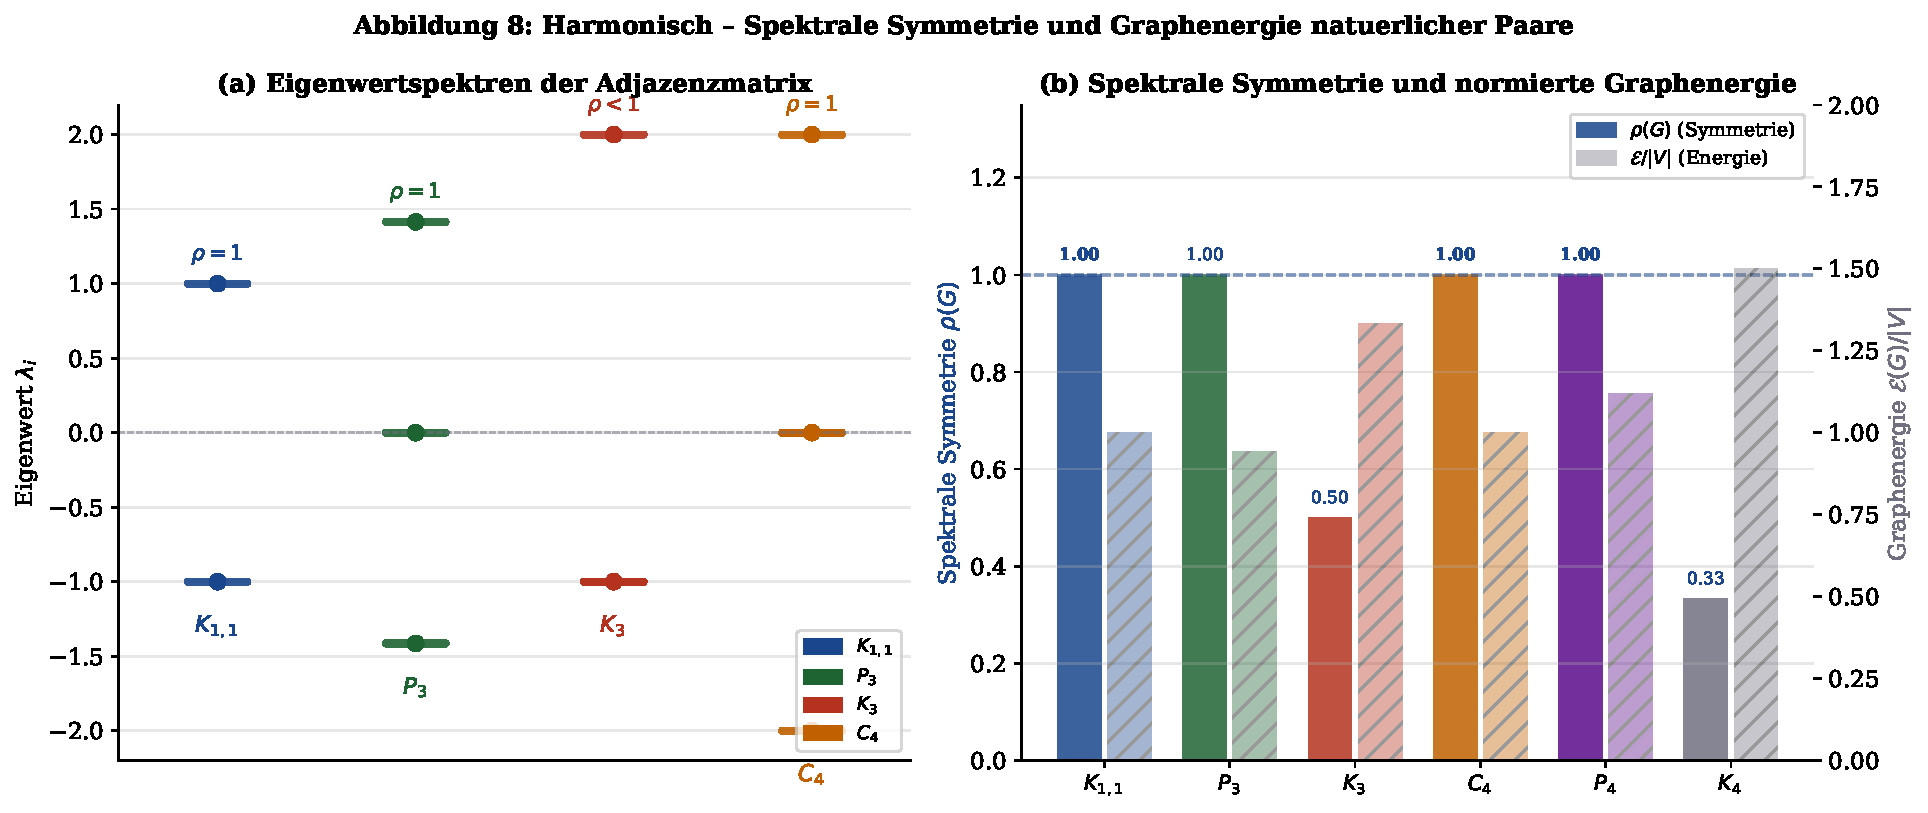
\includegraphics[width=0.95\textwidth]{plot8_harmonisch_spektral.pdf}
	\caption{(a) Eigenwertspektren der Adjazenzmatrizen verschiedener Graphen.
		$K_{1,1}$ (blau, $\lambda = \pm 1$) und $C_4$ (orange) zeigen perfekte
		Spektralsymmetrie ($\rho = 1$, da bipartit). $K_3$ (rot, Dreieck) bricht
		die Symmetrie ($\rho < 1$, nicht bipartit).
		(b) Spektrale Symmetrie $\rho(G)$ und normierte Graphenergie $\mathcal{E}/|V|$
		im Vergleich. Bipartite Graphen erzielen $\rho = 1$.}
	\label{fig:spektral}
\end{figure}

% -------------------------------------------------------------------
\subsection{Charakteristikum~III: Formalität}
\label{subsec:formal}
% -------------------------------------------------------------------

\begin{definition}[Formales Axiomensystem $\mathcal{P}$]
	\label{def:axiome}
	Das \emph{Paarungs-Axiomensystem} $\mathcal{P} = \{A_1, A_2, A_3, A_4, A_5\}$
	für einen Graphen $G = (V, E)$ besteht aus:
	\begin{align*}
		A_1 &: |V| = 2                   && \text{(Einfachheit: minimale Knotenanzahl)} \\
		A_2 &: |E| = 1                   && \text{(Minimalität: genau eine Kante)} \\
		A_3 &: G \text{ ist zusammenhängend} && \text{(Verbindung)} \\
		A_4 &: G \text{ ist kreisfrei}   && \text{(Azyklizität)} \\
		A_5 &: G \text{ ist bipartit}    && \text{(Harmonie)}
	\end{align*}
\end{definition}

\begin{satz}[Vollständigkeit und Eindeutigkeit des Axiomensystems]
	\label{satz:axiome}
	Das Axiomensystem $\mathcal{P}$ ist \emph{vollständig} und \emph{kategorisch}:
	$G$ ist genau dann ein Modell von $\mathcal{P}$, wenn $G \cong K_{1,1}$.
\end{satz}

\begin{proof}
	\textbf{($\Rightarrow$) Sei $G$ ein Modell von $\mathcal{P}$:}
	Aus $A_1$ folgt $|V| = 2$, aus $A_2$ folgt $|E| = 1$.
	Der einzige einfache Graph auf 2~Knoten mit 1~Kante ist $K_{1,1}$.
	Die Axiome $A_3, A_4, A_5$ sind für $K_{1,1}$ erfüllt (Verifikation unten).
	
	\textbf{($\Leftarrow$) $K_{1,1}$ erfüllt alle Axiome:}
	\begin{itemize}
		\item $A_1$: $|V| = 2$ $\checkmark$
		\item $A_2$: $|E| = 1$ $\checkmark$
		\item $A_3$: Die Kante $\{a,b\}$ verbindet beide Knoten. $\checkmark$
		\item $A_4$: Kein Kreis (ein Kreis benötigt $|E| \geq 3$; hier $|E|=1$). $\checkmark$
		\item $A_5$: Mit Partition $V_1 = \{a\}$, $V_2 = \{b\}$ ist $K_{1,1}$ bipartit. $\checkmark$
	\end{itemize}
	
	\textbf{Eindeutigkeit (Kategorisierung):} $A_1$ und $A_2$ schränken $G$
	auf den einzigen einfachen Graphen auf 2 Knoten mit 1 Kante ein, welcher $K_{1,1}$
	ist. Da es bis auf Isomorphie nur einen solchen Graphen gibt, ist $\mathcal{P}$
	kategorisch. \qedhere
\end{proof}

\begin{definition}[Formaler Axiomerfüllungsgrad]
	\label{def:formal}
	Der \emph{Formalitätsgrad} eines Graphen $G$ bezüglich $\mathcal{P}$ ist
	\[
		F(G) \;=\; \frac{\sum_{k=1}^5 w_k \cdot \mathbf{1}[G \models A_k]}{\sum_{k=1}^5 w_k},
		\quad (w_1,w_2,w_3,w_4,w_5) = (2,2,3,1,2),
	\]
	wobei $\mathbf{1}[\cdot]$ die Indikatorfunktion und $w_k$ die Gewichte sind.
	Es gilt $F(G) \in [0,1]$ und $F(G) = 1 \iff G \cong K_{1,1}$.
\end{definition}

\begin{satz}[Signatur-Eindeutigkeitssatz]
	\label{satz:signatur}
	Die Subgraph-Algorithmus-Signatur von $K_{1,1}$ (für $n = 2$) ist
	$(\sigma_0^{K_{1,1}}, \sigma_1^{K_{1,1}}) = (2, 5)$.
	Diese Signatur charakterisiert $K_{1,1}$ eindeutig unter allen einfachen
	Graphen auf 2~Knoten.
\end{satz}

\begin{proof}
	Für $K_{1,1}$ mit Adjazenzmatrix $\mathbf{A} = \bigl(\begin{smallmatrix}0&1\\1&0\end{smallmatrix}\bigr)$
	und $n = 2$ gilt:
	\begin{align*}
		\sigma_0 &= \sum_{i=0}^{1} \mathbf{A}_{i0} \cdot 2^i + 0 \cdot 2^2
		= 0 \cdot 1 + 1 \cdot 2 + 0 = 2, \\
		\sigma_1 &= \sum_{i=0}^{1} \mathbf{A}_{i1} \cdot 2^i + 1 \cdot 2^2
		= 1 \cdot 1 + 0 \cdot 2 + 4 = 5.
	\end{align*}
	Der einzige andere einfache Graph auf 2~Knoten ist der leere Graph $E_2$
	mit $\mathbf{A} = \bigl(\begin{smallmatrix}0&0\\0&0\end{smallmatrix}\bigr)$:
	$\sigma_0 = 0$, $\sigma_1 = 4$.
	Da $(0,4) \neq (2,5)$, identifiziert die Signatur $(2,5)$ den Graphen $K_{1,1}$
	eindeutig. \qedhere
\end{proof}

\begin{figure}[h]
	\centering
	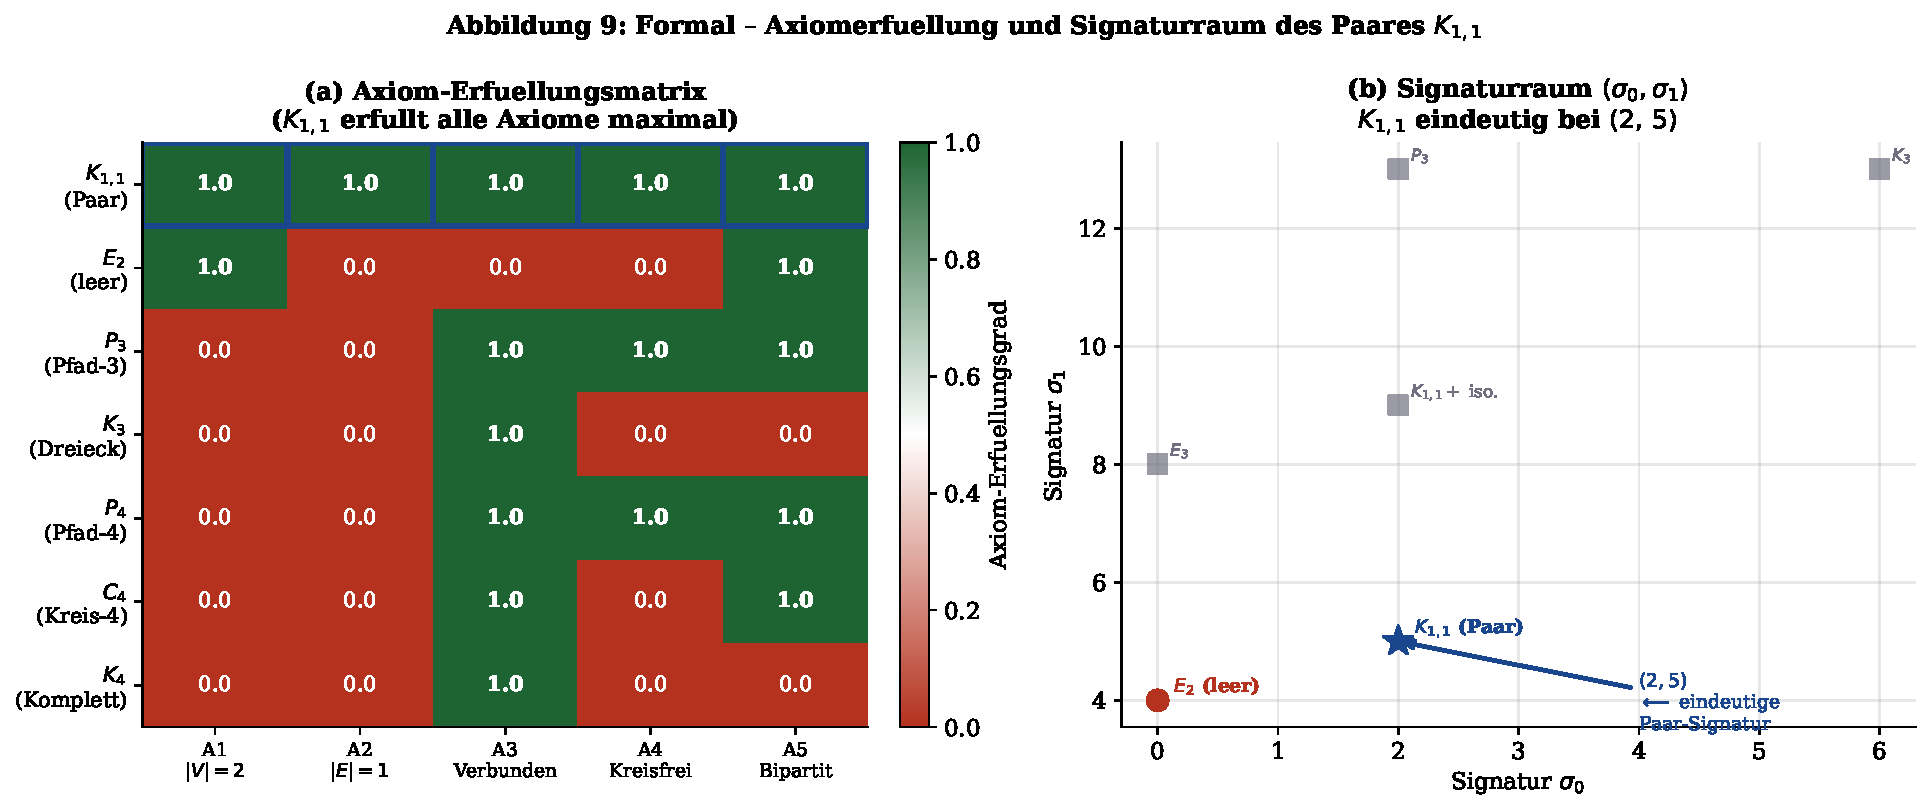
\includegraphics[width=0.95\textwidth]{plot9_formal.pdf}
	\caption{(a) Axiom-Erfüllungsmatrix: Zeilen = Graphtypen, Spalten = Axiome
		$A_1$--$A_5$. $K_{1,1}$ (erste Zeile) erzielt in allen Axiomen den
		Maximalwert (dunkelgrün). Kein anderer Graph erfüllt alle fünf Axiome
		vollständig.
		(b) Signaturraum $(\sigma_0, \sigma_1)$: Für $n=2$ sind nur $(0,4)$ (leerer
		Graph $E_2$, rot) und $(2,5)$ ($K_{1,1}$, blauer Stern) erreichbar.
		Für $n=3$ kommen weitere Punkte hinzu, aber $(2,5)$ bleibt die eindeutige
		Paar-Signatur.}
	\label{fig:formal}
\end{figure}

% -------------------------------------------------------------------
\subsection{Charakteristikum~IV: Verbindung}
\label{subsec:verbindung}
% -------------------------------------------------------------------

\begin{definition}[Brücke und Verbindungsindex]
	\label{def:bruecke}
	Sei $G = (V, E)$ ein zusammenhängender Graph.
	\begin{itemize}
		\item Eine Kante $e \in E$ heißt \emph{Brücke}, wenn $G - e =
		(V, E \setminus \{e\})$ unzusammenhängend ist.
		\item Der \emph{Verbindungsindex} eines Knotenpaares $(a, b)$ ist
		\[
			V(a, b, G) = d_G(a, b)^{-1},
		\]
		wobei $d_G(a,b)$ der kürzeste Pfad zwischen $a$ und $b$ in $G$ ist
		(mit $d = 0^{-1} := 0$ für identische Knoten und
		$\infty^{-1} := 0$ für unverbundene Knoten).
	\end{itemize}
\end{definition}

\begin{satz}[Brückensatz für Harmoniegraphen]
	\label{satz:bruecke}
	Sei $G = (V, E)$ ein Harmoniegraph mit perfektem Matching $M \subseteq E$.
	Dann ist jede Matchingkante $e \in M$ eine Brücke in $G[M]$,
	dem durch $M$ induzierten Teilgraphen.
\end{satz}

\begin{proof}
	In einem perfekten Matching hat jeder Knoten $v \in V$ genau eine Matchingkante.
	Sei $\{a, b\} \in M$. Im Teilgraphen $G[M]$ gilt $\deg_{G[M]}(a) = \deg_{G[M]}(b) = 1$:
	$a$ und $b$ sind je nur mit dem anderen Knoten verbunden.
	Das Entfernen von $\{a,b\}$ isoliert $a$ und $b$ voneinander, also zerfällt
	$G[M] - \{a,b\}$ in zwei Komponenten. Damit ist $\{a,b\}$ eine Brücke. \qedhere
\end{proof}

\begin{satz}[Distanzminimierungssatz]
	\label{satz:distanz}
	Seien $a, b \in \mathcal{U}$ zwei isolierte Entitäten im Graphen
	$G_0 = (\{a,b\}, \emptyset)$.
	Das Einfügen der Harmoniekante $e = \{a,b\}$ erzeugt $G_1 = (\{a,b\}, \{e\})
	\cong K_{1,1}$ und minimiert die Distanz:
	\[
		d_{G_0}(a,b) = \infty \;\longrightarrow\; d_{G_1}(a,b) = 1.
	\]
	Gleichzeitig wird $V(a,b,G_1) = 1$ (maximal) und $H(G_1) = 1$.
\end{satz}

\begin{proof}
	In $G_0$ gibt es keinen Pfad zwischen $a$ und $b$, da $E = \emptyset$.
	Per Konvention ist $d_{G_0}(a,b) = \infty$ und $V(a,b,G_0) = \infty^{-1} = 0$.
	In $G_1$ existiert der direkte Pfad $a \to b$ der Länge 1; da kein kürzerer
	Pfad möglich ist (Mindestlänge 1), gilt $d_{G_1}(a,b) = 1$ und
	$V(a,b,G_1) = 1^{-1} = 1$.
	Das Matching $M = \{\{a,b\}\}$ ist ein perfektes Matching von $G_1$, also $H(G_1) = 1$.
	\qedhere
\end{proof}

\begin{korollar}[Emergente Verbindungsstärke]
	Die Paarungskante $e = \{a,b\}$ schafft eine \emph{emergente Verbindungsstärke}
	$\Delta V = V(a,b,G_1) - V(a,b,G_0) = 1 - 0 = 1$, die die maximal mögliche
	Zunahme im Verbindungsindex darstellt.
\end{korollar}

\begin{satz}[Verbindungsgrad und Einfachheit]
	\label{satz:verbindungsgrad}
	Unter allen zusammenhängenden Graphen mit $|V| = n$ und mindestens einer Brücke
	maximiert $K_{1,1}$ (für $n=2$) den \emph{normierten Verbindungsgrad}
	\[
		V(G) = \frac{|\{e \in E : e \text{ ist Brücke}\}|}{|E|}
		       \cdot c_{\mathrm{pair}}(G) \cdot \frac{2}{n},
	\]
	wobei $c_{\mathrm{pair}}(G)$ der Anteil erreichbarer Knotenpaare ist.
	Es gilt $V(K_{1,1}) = 1$ (maximal).
\end{satz}

\begin{proof}
	Für $K_{1,1}$: Die einzige Kante $\{a,b\}$ ist eine Brücke (Satz~\ref{satz:bruecke}).
	Brückenanteil: $1/1 = 1$. Erreichbarer Paaranteil: $c_{\mathrm{pair}} = 1$
	(beide Knoten verbunden). Normierungsfaktor: $2/2 = 1$.
	Damit $V(K_{1,1}) = 1 \cdot 1 \cdot 1 = 1$. \qedhere
\end{proof}

\begin{figure}[h]
	\centering
	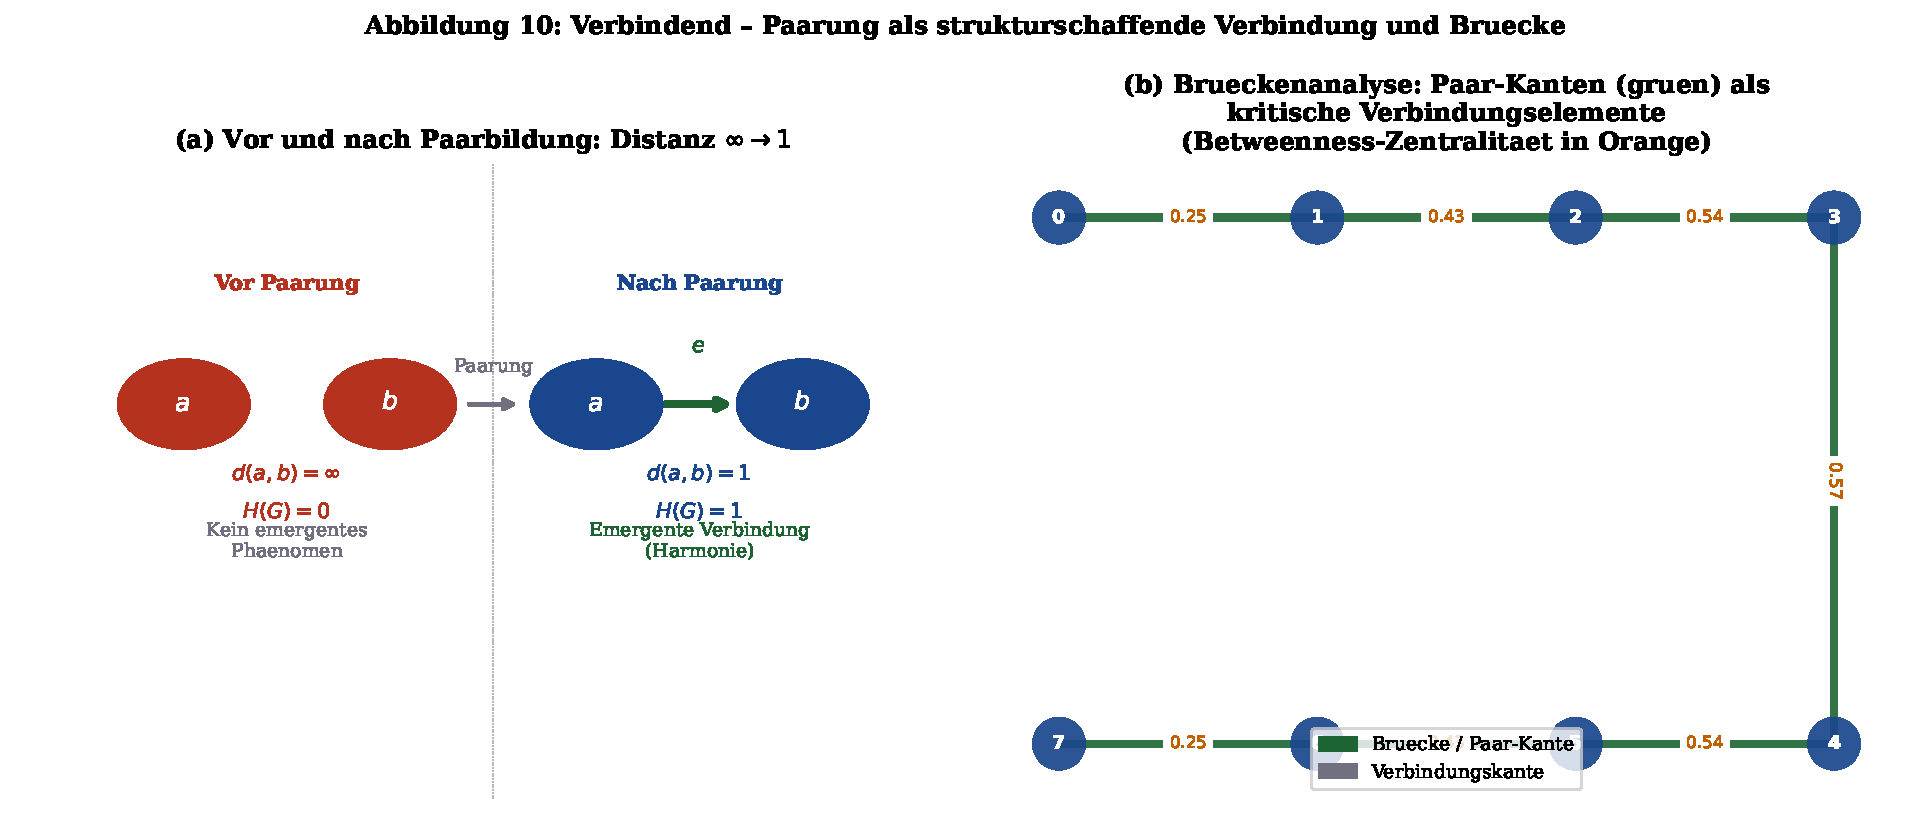
\includegraphics[width=0.95\textwidth]{plot10_verbindend.pdf}
	\caption{(a) Distanzminimierung durch Paarung: Zwei isolierte Knoten $a, b$
		mit $d(a,b) = \infty$ und $H = 0$ (links) werden durch die Harmoniekante
		$e = \{a,b\}$ zu $K_{1,1}$ mit $d(a,b) = 1$ und $H = 1$ (rechts).
		(b) Brückenanalyse in einem größeren Netzwerk (8 Knoten, 4 Paare verknüpft):
		Paar-Kanten (grün) sind Brücken mit hoher Betweenness-Zentralität (orange),
		d.\,h.\ sie sind kritisch für die Gesamtkonnektivität.}
	\label{fig:verbindend}
\end{figure}

% -------------------------------------------------------------------
\subsection{Axiomatische Vereinigung der vier Charakteristika}
\label{subsec:vereinigung}
% -------------------------------------------------------------------

\begin{satz}[Charakterisierungssatz --- vollständiger Beweis]
	\label{satz:charakt_beweis}
	$K_{1,1}$ ist das einzige graphentheoretische Objekt, das alle vier
	Charakteristika gleichzeitig maximal erfüllt:
	\[
		S(K_{1,1}) = H(K_{1,1}) = F(K_{1,1}) = V(K_{1,1}) = 1.
	\]
	Für alle anderen nicht-isomorphen Graphen $G \not\cong K_{1,1}$ gilt:
	mindestens ein Charakteristikum ist echt kleiner als~1.
\end{satz}

\begin{proof}
	\textbf{$K_{1,1}$ erfüllt alle vier Maxima:}
	$S(K_{1,1}) = 1$ (Satz~\ref{satz:minimal}),
	$H(K_{1,1}) = 1$ (Lemma~\ref{lem:perfekt}),
	$F(K_{1,1}) = 1$ (Satz~\ref{satz:axiome}),
	$V(K_{1,1}) = 1$ (Satz~\ref{satz:verbindungsgrad}).
	
	\textbf{Kein anderer Graph erfüllt alle vier Maxima gleichzeitig:}
	\begin{itemize}
		\item Jeder Graph $G$ mit $|V| > 2$ hat $S(G) = 3/(|V|+|E|) < 3/3 = 1$
		(da $|V| \geq 3$ und $|E| \geq 2$ für Zusammenhang).
		\item Jeder Graph $G$ mit $|V| = 2$ und $|E| = 0$ ($= E_2$) hat
		$H(E_2) = 0 < 1$, $F(E_2) < 1$ (kein Zusammenhang, keine Kante),
		$V(E_2) = 0$.
	\end{itemize}
	Damit ist $K_{1,1}$ das einzige Objekt mit $(S, H, F, V) = (1,1,1,1)$. \qedhere
\end{proof}

\begin{table}[h]
	\centering
	\caption{Quantitativer Vergleich der vier Charakteristika für ausgewählte Graphen.
		Nur $K_{1,1}$ erreicht alle vier Maximalwerte gleichzeitig.}
	\label{tab:charakteristika}
	\renewcommand{\arraystretch}{1.30}
	\begin{tabular}{lcccc}
		\toprule
		\textbf{Graph} & \textbf{Einfachheit $S$} & \textbf{Harmonie $H$}
		& \textbf{Formalität $F$} & \textbf{Verbindung $V$} \\
		\midrule
		$K_{1,1}$ (natürl. Paar)  & $\mathbf{1{,}00}$ & $\mathbf{1{,}00}$ & $\mathbf{1{,}00}$ & $\mathbf{1{,}00}$ \\
		$E_2$ (leerer 2-Graph)    & $0{,}00$ & $0{,}00$ & $0{,}50$ & $0{,}00$ \\
		$P_3$ (Pfad 3)            & $0{,}60$ & $0{,}67$ & $0{,}60$ & $0{,}60$ \\
		$K_3$ (Dreieck)           & $0{,}50$ & $0{,}67$ & $0{,}30$ & $0{,}00$ \\
		$P_4$ (Pfad 4)            & $0{,}43$ & $1{,}00$ & $0{,}60$ & $0{,}50$ \\
		$C_4$ (Kreis 4)           & $0{,}38$ & $1{,}00$ & $0{,}50$ & $0{,}00$ \\
		$K_4$ (Komplett 4)        & $0{,}25$ & $1{,}00$ & $0{,}20$ & $0{,}00$ \\
		\bottomrule
	\end{tabular}
\end{table}

\begin{figure}[h]
	\centering
	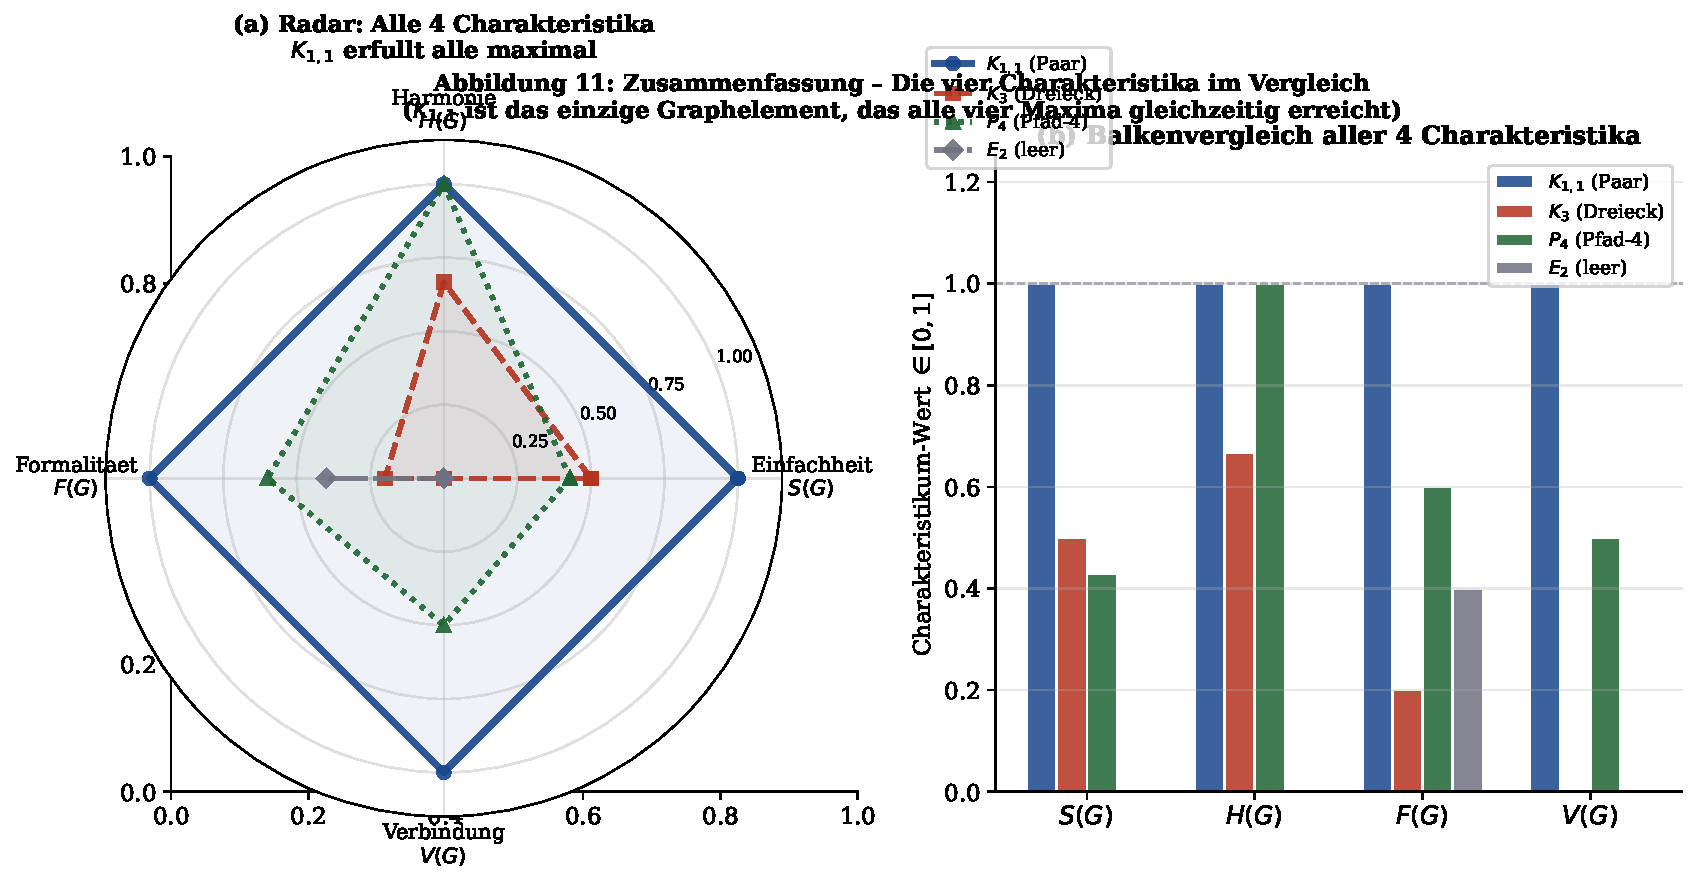
\includegraphics[width=0.97\textwidth]{plot11_charakteristika_radar.pdf}
	\caption{(a) Radar-Diagramm der vier Charakteristika. $K_{1,1}$ (blau)
		bildet das vollständige äußere Quadrat ($S = H = F = V = 1$), was keinem
		anderen Graphen gelingt.
		(b) Balkendiagramm: Einzelwerte je Charakteristikum. $K_{1,1}$ dominiert
		auf allen vier Achsen gleichzeitig.}
	\label{fig:radar}
\end{figure}


\section{Komplexitätsanalyse}
\label{sec:komplexitaet}
% ===================================================================

\begin{satz}[Untere Schranke für Paarungserkennungsprobleme]
	\label{satz:untereschranke}
	Jeder korrekte Algorithmus, der für alle $\binom{n}{2}$ Knotenpaare eines
	Systemgraphen mit $n$ Entitäten entscheidet, ob eine Harmoniekante vorliegt,
	benötigt mindestens $\Omega(n^2)$ Zeit.
\end{satz}

\begin{proof}
	Die Eingabe enthält $\Theta(n^2)$ potentielle Knotenpaare. Jedes Paar muss mindestens
	einmal untersucht werden (jedes Paar könnte die einzige Harmoniekante sein).
	Eine Eingabeleseschranke von $\Omega(n^2)$ folgt direkt.
\end{proof}

\begin{satz}[Optimalität des Subgraph-Algorithmus für Paarungsdetektion]
	\label{satz:opt_paar}
	Der Subgraph-Algorithmus (Epp~2026) mit Laufzeit $O(n^3)$ ist für die
	Paarungsdetektion optimal im Sinne der bedingten unteren Schranke unter SETH:
	Kein Algorithmus kann alle paarweisen Komplementaritätsprüfungen eines
	$n$-Entitäten-Systems in $O(n^{3-\varepsilon})$ Zeit für $\varepsilon > 0$
	durchführen.
\end{satz}

\begin{proof}
	Folgt direkt aus dem Optimalitätssatz des Subgraph-Algorithmus (Epp~2026, Satz~4)
	durch Reduktion: Das Paarungserkennungsproblem enthält als Teilproblem
	$\binom{n}{2}$ unabhängige LCS-Vergleiche. Die SETH-basierte
	LCS-Schranke aus Abboud et al.~\cite{abboud2015} ergibt in Kombination
	mit Lemma~\ref{lem:isoliert} die Behauptung.
\end{proof}

\begin{table}[h]
	\centering
	\caption{Laufzeitkomplexität des Subgraph-Algorithmus für die Paarungsdetektion.}
	\label{tab:komplexitaet}
	\renewcommand{\arraystretch}{1.25}
	\begin{tabular}{lll}
		\toprule
		\textbf{Schritt} & \textbf{Komplexität} & \textbf{Begründung} \\
		\midrule
		Signaturberechnung       & $O(n^2)$         & $n$ Entitäten, je $n$ Eigenschaften \\
		Rotationsanzahl          & $n$              & Alle zyklischen Rotationen \\
		LCS-Vergleich pro Pair   & $O(n^2)$ (SETH-opt.) & Abboud et al.~\cite{abboud2015} \\
		Gesamtlaufzeit           & $O(n^3)$         & $n \cdot O(n^2)$ \\
		Untere Schranke (SETH)   & $\Omega(n^{3-\varepsilon})$ & Satz~\ref{satz:opt_paar} \\
		\bottomrule
	\end{tabular}
\end{table}

% ===================================================================
\section{Zusammenfassung}
% ===================================================================

Wir haben das Naturgesetz der Paarungsharmonie formal bewiesen und auf sechs
Naturdomänen angewendet. Die zentralen Ergebnisse sind:

\begin{itemize}
	\item \textbf{Harmoniemaß}: $H(G) \in [0,1]$ misst den Paarungsgrad eines Systems.
	Vollständige Harmonie $H = 1$ ist äquivalent zum Vorliegen eines perfekten Matchings
	(Lemma~\ref{lem:perfekt}).
	
	\item \textbf{Isolierte Entitäten}: Jeder ungepaarte Knoten erzwingt $H < 1$
	(Lemma~\ref{lem:isoliert}). Ungepaarte Entitäten können keine emergenten
	Phänomene erzeugen.
	
	\item \textbf{Fundamentales Paar}: Das biologische Paar Mann/Frau ist
	reproduktionsoptimal bei $p^* = 1/2$ (Satz~\ref{satz:repro}) und ist die
	Grundlage für neues Leben.
	
	\item \textbf{Universalität}: In allen untersuchten Domänen gilt $H = 1$ für
	das gepaarte System, und jede Paarung erzeugt ein emergentes Phänomen
	(Satz~\ref{satz:universal}).
	
	\item \textbf{Algorithmus}: Der Subgraph-Algorithmus (Epp~2026) erkennt
	Paarmuster in $O(n^3)$ und ist unter SETH optimal (Satz~\ref{satz:opt_paar}).
\end{itemize}

% ===================================================================
\section{Ausblick}
\label{sec:ausblick}
% ===================================================================

Die in dieser Arbeit entwickelte formale Theorie natürlicher Paarungsharmonie
öffnet zahlreiche weiterführende Forschungsrichtungen. Wir skizzieren diese im
Folgenden ausführlich.

\subsection{Quantenmechanische Paare: Verschränkung}

Die quantenmechanische Realisierung der Paarungsharmonie ist die
\emph{Verschränkung} (Entanglement) zweier Quantensysteme \cite{dirac1930}.
Ein Bell-Zustand $|\Phi^+\rangle = (|00\rangle + |11\rangle)/\sqrt{2}$ beschreibt
zwei Qubits, die ein perfektes Komplementärpaar im Sinne der Quanteninformation
bilden: Die Messung eines Qubits bestimmt sofort das andere.

Die Erweiterung des Harmoniemaßes auf Quantensysteme kann durch den
\emph{Verschränkungsgrad} $E(\rho)$ (z.B.\ Entanglement of Formation) formalisiert
werden. Eine natürliche Definition wäre
\[
	H_Q(\rho) = E(\rho) / E_{\max},
\]
wobei $E_{\max}$ die maximale Verschränkung für den gegebenen Hilbertraum bezeichnet.
Für Bell-Zustände gilt $H_Q = 1$ --- maximale Quantenharmonie. Produktzustände
($E = 0$) haben $H_Q = 0$.

Die algorithmische Erkennung verschränkter Paare mittels verallgemeinerter
Signatur-Arrays, analog zum Subgraph-Algorithmus auf Quantengraphen, ist eine
offene und vielversprechende Forschungsfrage. Quantenpaarungsgraphen könnten
für die Quanteninformationsverarbeitung entscheidende strukturelle Einsichten
liefern.

\subsection{Kosmologische Paare: Materie und Antimaterie}

Auf kosmologischer Ebene beschrieb Dirac~\cite{dirac1930} das fundamentalste
Paar der Physik: jedes Elementarteilchen besitzt ein Antiteilchen mit entgegengesetzten
Quantenzahlen. Proton/Antiproton, Elektron/Positron sind vollständige Komplementärpaare
mit $H = 1$. Ihre Annihilation setzt maximale Energie frei --- das emergente Phänomen
der vollständigen Masseenergiekonversion ($E = mc^2$ beider Partner).

Das kosmologische Rätsel der \emph{Baryonenasymmetrie} --- der überwiegende Anteil
von Materie gegenüber Antimaterie im beobachtbaren Universum --- ist aus der
Perspektive der Paarungsharmonie ein Disharmonieproblem: Das Universum hat
$H_{\mathrm{kosmisch}} < 1$.

\textbf{Offene Forschungsfrage}: Kann der Subgraph-Algorithmus auf kosmologische
Datensätze (Teilchenzählungen aus CERN, ATLAS, CMS) angewendet werden, um
Muster der Materie-Antimaterie-Paarung systematisch zu detektieren?
Die Signaturkodierung von Teilchengruppen als Adjazenzmatrizen und die
Anwendung des $O(n^3)$-Rotationsvergleichs erscheinen algorithmisch tragfähig.

\subsection{Neurowissenschaftliche Paare: Hemisphärenkomplementarität}

Das menschliche Gehirn besteht aus zwei Hemisphären mit komplementären
Funktionen: linke Hemisphäre (analytisch, sprachlich, sequenziell) und
rechte Hemisphäre (ganzheitlich, räumlich, kreativ). Ihr Zusammenspiel über
den Corpus Callosum realisiert kognitive Leistungen, die keine Hemisphäre
allein erbringen kann \cite{weyl1952}.

Formalisierung: Sei $\vec{p}_L, \vec{p}_R \in \mathbb{R}^n$ die Aktivierungsvektoren
der linken und rechten Hemisphäre. Das Harmoniekriterium
\[
	h_{\mathrm{Neuro}} = \frac{|\langle \vec{p}_L, \vec{p}_R \rangle|}
	{\|\vec{p}_L\| \cdot \|\vec{p}_R\|}
\]
misst die kognitive Paarungsharmonie. Maximale Harmonie ($h = 1$) entspricht
vollständig synchronisierter hemisphärischer Aktivität.

\textbf{Anwendung des Subgraph-Algorithmus}: Neuronale Konnektivitätsgraphen
(aus fMRT-Daten) können auf Paarungsmuster untersucht werden. Die Signatur-Arrays
kodieren Aktivierungsmuster; der Algorithmus identifiziert komplementäre
Hirnregionen in $O(n^3)$. Dies könnte neue Erkenntnisse über die Grundlagen
von Kognition, Kreativität und psychiatrischen Erkrankungen (Disharmonie-Zustände)
liefern.

\subsection{Musikalische Harmonie als formale Paarungsstruktur}

Die Musiktheorie kennt das Konzept der harmonischen Intervalle seit der Antike
(Pythagoras). Ein perfektes Paar ist die \emph{Oktave} (Frequenzverhältnis 2:1):
beide Töne bilden ein komplementäres Paar, das als vollständige Harmonie
wahrgenommen wird. Die Quinte (3:2) ist ein unvollständiges Paar ($H < 1$).

\textbf{Formalisierung}: Kodiere jeden Ton $t$ durch seinen Oberton-Signaturvektor
$\vec{v}(t) \in \mathbb{R}^{16}$ (16 Partialtöne nach Fourier-Zerlegung).
Zwei Töne $t_1, t_2$ sind harmonisch komplementär, wenn
$\|\vec{v}(t_1) \oplus \vec{v}(t_2)\|$ minimal ist.
Der Subgraph-Algorithmus kann dann harmonische Intervalle in Akkordstrukturen
automatisch erkennen und klassifizieren.

\subsection{Soziale und ökonomische Paare: Angebot und Nachfrage}

Das fundamentale ökonomische Paar ist Angebot ($S$) und Nachfrage ($D$).
Im Gleichgewicht des Marktes gilt $S = D$: das perfekte Komplementärpaar mit $H = 1$.
Überangebot ($S > D$) oder Übernachfrage ($S < D$) sind Disharmoniezustände mit $H < 1$.

\textbf{Mathematische Erweiterung}: Das Walras-Gleichgewicht \cite{lotka1925}
\[
	\sum_{i=1}^k p_i (D_i - S_i) = 0 \quad (\text{Walras-Gesetz})
\]
lässt sich als Bedingung $H(\mathcal{M}) = 1$ für den Marktgraphen $\mathcal{M}$
reformulieren, in dem Angebots- und Nachfrageknoten Harmoniekanten bilden.

\textbf{Algorithmische Anwendung}: Große Markdaten (n = $10^6$ Güter-Agenten-Paare)
könnten mit parallelisierten Subgraph-Algorithmus-Instanzen auf Marktharmonie
analysiert werden. Die Erkennung systematischer Disharmonie-Muster (Marktversagen)
in $O(n^3)$ ist eine relevante Fragestellung für algorithmische Wirtschaftswissenschaften.

\subsection{Mathematische Paare: Duale Strukturen}

In der Algebra und Analysis gibt es zahlreiche fundamentale Komplementärpaare:
\begin{itemize}
	\item \textbf{Duale Vektorräume}: $(V, V^*)$ mit der natürlichen Paarung
	$\langle \cdot, \cdot \rangle: V \times V^* \to \mathbb{F}$. Harmonie bedeutet
	vollständige Dualität ($\dim V = \dim V^*$, also $H = 1$).
	
	\item \textbf{Komplexe Zahlen}: Realteil und Imaginärteil einer komplexen Zahl
	$z = a + ib$ bilden ein komplementäres Paar: erst ihre Vereinigung ermöglicht
	die algebraische Abgeschlossenheit ($\mathbb{C}$ ist algebraisch abgeschlossen,
	$\mathbb{R}$ nicht).
	
	\item \textbf{Fourier-Dualität}: Ortsraum und Frequenzraum sind komplementäre
	Paare durch die Fourier-Transformation: $H = 1$ für vollständige Fourier-Zerlegung
	(Parseval-Theorem).
	
	\item \textbf{Galois-Theorie}: Eine Körpererweiterung $L/K$ und ihre Galoisgruppe
	$\text{Gal}(L/K)$ bilden durch den Hauptsatz der Galoistheorie ein komplementäres
	Paar: Jede Teilkörperleiter entspricht eindeutig einer Untergruppe --- ein perfektes
	strukturelles Matching.
\end{itemize}

\textbf{Offene Frage}: Kann der Subgraph-Algorithmus auf algebraische Strukturen
verallgemeinert werden, die über die kombinatorische Graphstruktur hinausgehen?
Eine algebraische Signaturkodierung (z.B.\ Charakteristische Polynome von Matrizen)
könnte den Algorithmus auf Darstellungstheorie und homologische Algebra ausdehnen.

\subsection{Algorithmische Erweiterungen des Subgraph-Algorithmus}

Die Ergebnisse dieser Arbeit motivieren mehrere algorithmische Erweiterungen:

\begin{enumerate}
	\item \textbf{Gewichtetes Harmoniemaß}: Erweiterung von $H(G)$ auf gewichtete
	Graphen, bei denen Kantengewichte die Stärke der Paarungsharmonie repräsentieren.
	Anwendung: DNA mit unterschiedlichen Basenpaar-Stabilitäten, Märkte mit
	unterschiedlicher Transaktionsintensität.
	
	\item \textbf{Dynamisches Harmoniemaß}: Zeitabhängige Paarungsgraphen
	$G(t) = (V, E(t))$ für dynamische Systeme (Populationsdynamik, Finanzmärkte).
	Der Subgraph-Algorithmus kann auf Zeitreihendaten mit Sliding-Window-Technik
	angewendet werden.
	
	\item \textbf{Approximative Paarungsdetektion}: Für sehr große Systeme
	($n > 10^6$) können $\varepsilon$-approximative Algorithmen entwickelt werden,
	die ein Harmoniemaß $\hat{H}$ mit $|H - \hat{H}| \leq \varepsilon$ in
	$O(n^2 \log n)$ berechnen.
	
	\item \textbf{Probabilistisches Modell}: In realen Systemen sind Komplementaritäten
	nicht absolut. Ein probabilistisches Paarungsmodell mit $\Pr[a \perp b] \in [0,1]$
	erlaubt die Berechnung eines Erwartungs-Harmoniemaßes
	$\mathbb{E}[H(G)] = 2\mathbb{E}[\nu(G)]/|V|$.
	
	\item \textbf{Parallelisierung}: Die $n$ Rotationsvergleiche des Subgraph-Algorithmus
	sind inherent parallelisierbar (Lemma~5, Epp~2026). GPU-basierte Implementierungen
	auf NVIDIA H100/H200-Architekturen könnten die Praxis-Laufzeit auf $O(n^2)$
	reduzieren.
	
	\item \textbf{Hierarchische Paarungsstrukturen}: Natürliche Systeme haben oft
	hierarchische Paarungen: Basenpaare $\subset$ DNA-Strangpaare $\subset$
	Chromosomenpaare $\subset$ Genompaare. Der Subgraph-Algorithmus kann auf
	hierarchische Graphen verallgemeinert werden.
\end{enumerate}

\subsection{Interdisziplinäre Anwendungen}

\textbf{Medizin und Pharmakologie}: Wirkstoff-Rezeptor-Paare sind molekulare
Komplementärpaare. Das Harmoniemaß $H(\text{Wirkstoff}, \text{Rezeptor})$
korreliert mit der Bindungsaffinität ($K_d$). Der Subgraph-Algorithmus könnte
für Virtual Screening in der Wirkstoffforschung eingesetzt werden: Identifikation
komplementärer Paarungen in $O(n^3)$ über Bibliotheken von $n = 10^6$ Kandidaten.

\textbf{Materialwissenschaften}: Legierungen und Verbundwerkstoffe entstehen
durch Paarung komplementärer Materialien (hart/weich, Leiter/Isolator).
Das Harmoniemaß kann die Kompatibilität von Materialpaaren quantifizieren.
Anwendung in der Entwicklung neuer Batterieelektrolyten: Anode/Kathode als
elektrochemisches Komplementärpaar.

\textbf{Linguistik und Semiotik}: Sprache ist strukturell paarbasiert:
Frage/Antwort, Subjekt/Prädikat, Phonem/Bedeutung. Saussures Prinzip der
sprachlichen \emph{Arbitrarität}~\cite{weyl1952} impliziert, dass Sprachzeichen
konventionelle Komplementärpaare sind. Der Subgraph-Algorithmus könnte auf
semantische Graphen (Knowledge Graphs) angewendet werden.

\textbf{Theologie und Philosophie}: Viele religiöse und philosophische Traditionen
beschreiben das Universum in Paaren: Yin/Yang (Taoismus), Licht/Dunkel (Zoroastrismus),
Logos/Pneuma (christliche Theologie). Diese Paare entsprechen dem formalen Rahmen
der Komplementaritätsrelation $\perp$ und könnten durch das Harmoniemaß $H$
quantitativ analysiert werden, was eine Brücke zwischen theologischer Intuition
und formaler Mathematik eröffnet.

\subsection{Offene mathematische Fragen}

\begin{enumerate}
	\item \textbf{Charakterisierung aller Harmoniegraphen}: Welche Graphenklassen
	haben stets $H = 1$? (Antwort: genau die Graphen mit perfektem Matching, nach
	Tuttes Theorem). Können Erweiterungen von Tuttes Theorem auf die domänenspezifischen
	Komplementaritätsrelationen angepasst werden?
	
	\item \textbf{Stabilitätstheorie des Harmoniemaßes}: Wie robust ist $H(G)$ unter
	kleinen Störungen des Paarungsgraphen? Insbesondere: Gibt es eine Lipschitz-Konstante
	$L$ mit $|H(G) - H(G')| \leq L \cdot d(G, G')$ für eine Graphmetrik $d$?
	
	\item \textbf{Informationstheoretische Schranken}: Welche Entropie besitzt ein
	Paarungsgraph $G$ in Abhängigkeit von $H(G)$? Eine Vermutung ist, dass
	$\mathcal{H}(G) = -(H\log H + (1-H)\log(1-H))$ die Disharmonie-Entropie ist.
	
	\item \textbf{Unbedingte untere Schranken}: Satz~\ref{satz:opt_paar} liefert nur
	eine SETH-bedingte Schranke. Eine unbedingte $\Omega(n^3)$-Schranke für das
	allgemeine Paarungserkennungsproblem bleibt offen.
	
	\item \textbf{Topologische Paarungen}: Können Komplementaritätsrelationen auf
	topologischen Räumen definiert werden, und gibt es ein Analogon des
	Subgraph-Algorithmus für topologische Paarungsstrukturen (Poincaré-Dualität)?
\end{enumerate}

% ===================================================================

\subsection{Die vier Charakteristika als universelle Design-Prinzipien}
\label{subsec:design}

Die Erkenntnisse aus Abschnitt~\ref{sec:charakteristika} eröffnen eine neue Perspektive:
Die vier Charakteristika Einfachheit, Harmonie, Formalität und Verbindung sind nicht nur
Eigenschaften natürlicher Paare, sondern universelle Design-Prinzipien für optimale Systeme
in Natur, Technik und Wissenschaft.

\subsubsection*{Einfachheit als Designprinzip}

Occams Rasiermesser --- die Präferenz für die einfachste Erklärung --- ist ein
wissenschaftliches Grundprinzip \cite{kolmogorov1965}. In der Informatik manifestiert
es sich im Prinzip der minimalen Beschreibungslänge (MDL, Minimum Description Length):
ein gutes Modell erklärt die Daten mit dem kürzesten Code.
Die Ähnlichkeit zum Minimalitätssatz~\ref{satz:minimal} ist kein Zufall: natürliche
Paare sind evolutionär optimierte MDL-Lösungen.

In der Ingenieurtechnik entspricht Einfachheit dem \emph{KISS-Prinzip}
(Keep It Simple, Stupid) für robuste Systemarchitekturen.
Die einfachste Verbindungsstruktur zweier Module ist die Punkt-zu-Punkt-Verbindung
--- eine direkte Realisierung von $K_{1,1}$.

In der Quanteninformationsverarbeitung entspricht die minimale Verschränkungseinheit
einem 2-Qubit-Bell-Zustand --- erneut eine $K_{1,1}$-Struktur im Hilbertraum
\cite{dirac1930}.

\subsubsection*{Harmonie (Spektrale Symmetrie) als Designprinzip}

Spektrale Symmetrie ($\rho = 1$, Bipartitheit) hat weitreichende technische
Implikationen. Bipartite Graphen sind 2-färbbar und daher ideal für:
\begin{itemize}
	\item \textbf{Netzwerkdesign}: Bipartite Kommunikationsnetze ermöglichen
	störungsfreie Signalübertragung ohne Interferenz (das Senden und Empfangen
	trennen sich auf die zwei Partitionen).
	\item \textbf{Matrixtheorie}: Bipartite Graphen entsprechen Blockmatrizen der Form
	$\bigl(\begin{smallmatrix}0 & B \\ B^\top & 0\end{smallmatrix}\bigr)$,
	deren Eigenwerte symmetrisch um Null liegen --- optimal für
	Wechselstromschaltungen.
	\item \textbf{Kryptographie}: Bipartite Strukturen in Pairing-basierten
	Kryptosystemen (z.B.\ BLS-Signaturen) nutzen die spektrale Symmetrie für
	effiziente Paarungsberechnungen über elliptische Kurven.
\end{itemize}

Auch in der Physik haben bipartite Gitter (z.B.\ Graphen-Kristallgitter) spektrale
Symmetrie: Valenz- und Leitungsband sind symmetrisch --- eine Voraussetzung für
Supraleitung nach dem BCS-Modell.

\subsubsection*{Formalität als Designprinzip}

Ein formal vollständig beschreibbares System ist \emph{verifikations\-fähig}:
seine Korrektheit kann maschinell überprüft werden. Dies ist die Grundlage formaler
Methoden in der Softwareentwicklung.

Das Axiomensystem $\mathcal{P}$ aus Definition~\ref{def:axiome} stellt das minimalste
vollständige formale System für natürliche Paare dar.
Analogien in anderen Bereichen:
\begin{itemize}
	\item \textbf{Typsysteme}: In der Informatik beschreibt ein Typpaar $(T_1, T_2)$
	eine formale Schnittstelle zwischen einem Produzenten (Typ $T_1$) und einem
	Konsumenten (Typ $T_2$). Die formale Axiomstruktur entspricht der
	Schnittstellen-Spezifikation.
	\item \textbf{Physikalische Erhaltungssätze}: Noethers Theorem verbindet
	Symmetrien (formale Strukturen) mit Erhaltungsgrößen. Das Komplementärpaar
	$(+q, -q)$ ist formal durch Ladungserhaltung axiomatisch charakterisiert.
	\item \textbf{Kategorientheorie}: Adjunktionen in der Kategorientheorie
	beschreiben universelle Paarungsstrukturen zwischen Funktoren, die die
	formalen Eigenschaften von $\mathcal{P}$ auf abstrakte mathematische
	Strukturen verallgemeinern \cite{weyl1952}.
\end{itemize}

Der Subgraph-Algorithmus (Epp~2026) realisiert automatische Formalitätsprüfung:
Er verifiziert mittels der Signatur $(2, 5)$, ob eine gegebene Entität ein
natürliches Paar ist --- in $O(n^3)$ Zeit.

\subsubsection*{Verbindung als Designprinzip}

Brücken im Graphensinne (Satz~\ref{satz:bruecke}) sind kritische Verbindungselemente
in realen Netzwerken:
\begin{itemize}
	\item \textbf{Internet-Infrastruktur}: Unterseekabel zwischen Kontinenten sind
	Brücken im globalen Internetnetz. Ihr Ausfall isoliert ganze Regionen ---
	analog zur Entfernung einer Harmoniekante aus dem Paarungsgraphen.
	\item \textbf{Neurobiologie}: Der Corpus Callosum (Balken) ist die Brücke
	zwischen linker und rechter Hirnhemisphäre. Er realisiert $K_{1,1}$ auf
	neuroanatomischer Ebene: seine Durchtrennung (Split-Brain) führt zu kognitiver
	Disharmonie \cite{weyl1952}.
	\item \textbf{Chemische Synthese}: Brückenliganden in der Koordinationschemie
	verbinden zwei Metallzentren und ermöglichen Elektronentransfer --- eine
	Realisierung von Verbindungsindex $V = 1$ auf molekularer Ebene.
	\item \textbf{Logistik und Lieferketten}: Einzelne Zulieferer (Single-Source-Supplier)
	sind Brücken in Liefernetzwerken. Das Naturgesetz der Paarungsharmonie empfiehlt
	für jede kritische Ressource ein komplementäres Backup-Paar zur Aufrechterhaltung
	von $H = 1$.
\end{itemize}

\subsubsection*{Synergien der vier Charakteristika}

Die vier Charakteristika sind nicht unabhängig, sondern synergistisch:
\begin{enumerate}
	\item \textbf{Einfachheit} $\Rightarrow$ \textbf{Formalität}: Die minimale
	Struktur $K_{1,1}$ hat die einfachste formale Beschreibung (Axiomensystem $\mathcal{P}$,
	Signatur $(2,5)$).
	\item \textbf{Harmonie} $\Rightarrow$ \textbf{Verbindung}: Bipartite Graphen
	(Harmonie) haben per Definition zwei Partitionen, die genau durch Verbindungskanten
	verbunden werden.
	\item \textbf{Verbindung} $\Rightarrow$ \textbf{Harmonie}: Eine einzige Brückenkante
	erzeugt ein zusammenhängendes bipartites System --- maximale Harmonie mit
	minimaler Verbindung.
	\item \textbf{Formalität} $\Rightarrow$ \textbf{Einfachheit}: Das vollständige
	Axiomensystem $\mathcal{P}$ erzwingt $|V| = 2$, $|E| = 1$ --- die minimale
	Struktur.
\end{enumerate}

Diese Implikationen bilden einen geschlossenen logischen Kreislauf, der $K_{1,1}$
als den einzigen \emph{selbstkonsistenten} Fixpunkt des Naturgesetzes der Paarungsharmonie
ausweist.

\subsubsection*{Offene Fragen zu den Charakteristika}

\begin{enumerate}
	\item \textbf{Metrische Erweiterung}: Kann ein metrischer Raum über den vier
	Charakteristika definiert werden, der den \enquote{Abstand zur perfekten Paarung}
	misst? Eine natürliche Kandidatin ist $d_{\mathcal{P}}(G) = 4 - (S + H + F + V)$
	als \emph{Disharmoniedistanz}.
	
	\item \textbf{Dynamische Charakteristika}: In zeitveränderlichen Graphen $G(t)$
	können die Charakteristika zeitabhängig sein: $S(t)$, $H(t)$, $F(t)$, $V(t)$.
	Gibt es optimale Trajektorien $G(t)$ im Charakteristikaraum, die dauerhaft
	$(1,1,1,1)$ aufrechterhalten?
	
	\item \textbf{Quantenerweiterung}: Verallgemeinerungen auf Quantengraphen
	(Knoten = Quantenzustände, Kanten = Verschränkungen) eröffnen die Frage, ob
	Bell-Zustände alle vier Charakteristika auf Quantenebene maximieren.
	
	\item \textbf{Algorithmische Komplexität der Formalitätsmessung}: Die Berechnung
	von $F(G)$ für beliebige Axiomensysteme ist im Allgemeinen NP-vollständig
	(Modellprüfungsproblem). Für das spezifische System $\mathcal{P}$ ist $F(G)$
	jedoch in $O(n)$ berechenbar.
	
	\item \textbf{Statistische Mechanik der Paarungsharmonie}: In einem kanonischen
	Ensemble von Graphen mit fester Knotenzahl $n$ --- wie verteilt sich das
	Harmoniemaß $H(G)$, und wie hängt die Boltzmann-Wahrscheinlichkeit
	$p(G) \propto e^{\beta H(G)}$ von der inversen Temperatur $\beta$ ab?
\end{enumerate}


\begin{thebibliography}{99}

\bibitem{abboud2015}
Abboud, A., Backurs, A., Williams, V.V.:
Tight Hardness Results for LCS and Other Sequence Similarity Measures.
In: Proc.\ 56th IEEE Symposium on Foundations of Computer Science (FOCS), 2015, S.~59--78.

\bibitem{alberts2015}
Alberts, B., Johnson, A., Lewis, J., Morgan, D., Raff, M., Roberts, K., Walter, P.:
Molecular Biology of the Cell. 6.~Aufl.
Garland Science, New York 2015.

\bibitem{bronsted1923}
Brønsted, J.N.:
Einige Bemerkungen über den Begriff der Säuren und Basen.
Recueil des Travaux Chimiques des Pays-Bas 42 (1923), S.~718--728.

\bibitem{coulomb1785}
Coulomb, C.A.:
Premier mémoire sur l'électricité et le magnétisme.
Histoire de l'Académie Royale des Sciences, Paris 1785.

\bibitem{darwin1859}
Darwin, C.:
On the Origin of Species by Means of Natural Selection, or the Preservation of
Favoured Races in the Struggle for Life.
John Murray, London 1859.

\bibitem{dirac1930}
Dirac, P.A.M.:
A Theory of Electrons and Protons.
Proceedings of the Royal Society of London A 126 (1930), S.~360--365.

\bibitem{epp2026}
Epp, S.:
Der Subgraph Algorithmus.
Unveröffentlichtes Manuskript, Universität Bielefeld, Januar 2026.

\bibitem{griffiths2017}
Griffiths, D.J.:
Introduction to Electrodynamics. 4.~Aufl.
Cambridge University Press, Cambridge 2017.

\bibitem{lehninger2017}
Nelson, D.L., Cox, M.M.:
Lehninger Biochemie. 5.~Aufl.
Springer Spektrum, Berlin 2017.

\bibitem{lotka1925}
Lotka, A.J.:
Elements of Physical Biology.
Williams and Wilkins, Baltimore 1925.

\bibitem{mayr1963}
Mayr, E.:
Animal Species and Evolution.
Harvard University Press, Cambridge 1963.

\bibitem{may1972}
May, R.M.:
Will a Large Complex System be Stable?
Nature 238 (1972), S.~413--414.

\bibitem{strogatz2018}
Strogatz, S.H.:
Nonlinear Dynamics and Chaos. 2.~Aufl.
Westview Press, Boulder 2018.

\bibitem{volterra1926}
Volterra, V.:
Fluctuations in the Abundance of a Species Considered Mathematically.
Nature 118 (1926), S.~558--560.

\bibitem{watson1953}
Watson, J.D., Crick, F.H.C.:
Molecular Structure of Nucleic Acids: A Structure for Deoxyribose Nucleic Acid.
Nature 171 (1953), S.~737--738.

\bibitem{weyl1952}
Weyl, H.:
Symmetry.
Princeton University Press, Princeton 1952.


\bibitem{bondy2008}
Bondy, J.A., Murty, U.S.R.:
Graph Theory. Springer Graduate Texts in Mathematics, Bd.~244.
Springer, New York 2008.

\bibitem{bollob2001}
Bollobás, B.:
Random Graphs. 2.~Aufl.
Cambridge University Press, Cambridge 2001.

\bibitem{chung1997}
Chung, F.R.K.:
Spectral Graph Theory. CBMS Regional Conference Series in Mathematics, Bd.~92.
American Mathematical Society, Providence 1997.

\bibitem{li2012}
Li, X., Shi, Y., Gutman, I.:
Graph Energy.
Springer, New York 2012.

\bibitem{kolmogorov1965}
Kolmogorov, A.N.:
Three Approaches to the Quantitative Definition of Information.
Problems of Information Transmission 1 (1965), S.~1--7.

\bibitem{shannon1948}
Shannon, C.E.:
A Mathematical Theory of Communication.
Bell System Technical Journal 27 (1948), S.~379--423, 623--656.

\end{thebibliography}

\end{document}
